\documentclass[twoside]{book}

% Packages required by doxygen
\usepackage{fixltx2e}
\usepackage{calc}
\usepackage{doxygen}
\usepackage[export]{adjustbox} % also loads graphicx
\usepackage{graphicx}
\usepackage[utf8]{inputenc}
\usepackage{makeidx}
\usepackage{multicol}
\usepackage{multirow}
\PassOptionsToPackage{warn}{textcomp}
\usepackage{textcomp}
\usepackage[nointegrals]{wasysym}
\usepackage[table]{xcolor}

% Font selection
\usepackage[T1]{fontenc}
\usepackage[scaled=.90]{helvet}
\usepackage{courier}
\usepackage{amssymb}
\usepackage{sectsty}
\renewcommand{\familydefault}{\sfdefault}
\allsectionsfont{%
  \fontseries{bc}\selectfont%
  \color{darkgray}%
}
\renewcommand{\DoxyLabelFont}{%
  \fontseries{bc}\selectfont%
  \color{darkgray}%
}
\newcommand{\+}{\discretionary{\mbox{\scriptsize$\hookleftarrow$}}{}{}}

% Page & text layout
\usepackage{geometry}
\geometry{%
  a4paper,%
  top=2.5cm,%
  bottom=2.5cm,%
  left=2.5cm,%
  right=2.5cm%
}
\tolerance=750
\hfuzz=15pt
\hbadness=750
\setlength{\emergencystretch}{15pt}
\setlength{\parindent}{0cm}
\setlength{\parskip}{0.2cm}
\makeatletter
\renewcommand{\paragraph}{%
  \@startsection{paragraph}{4}{0ex}{-1.0ex}{1.0ex}{%
    \normalfont\normalsize\bfseries\SS@parafont%
  }%
}
\renewcommand{\subparagraph}{%
  \@startsection{subparagraph}{5}{0ex}{-1.0ex}{1.0ex}{%
    \normalfont\normalsize\bfseries\SS@subparafont%
  }%
}
\makeatother

% Headers & footers
\usepackage{fancyhdr}
\pagestyle{fancyplain}
\fancyhead[LE]{\fancyplain{}{\bfseries\thepage}}
\fancyhead[CE]{\fancyplain{}{}}
\fancyhead[RE]{\fancyplain{}{\bfseries\leftmark}}
\fancyhead[LO]{\fancyplain{}{\bfseries\rightmark}}
\fancyhead[CO]{\fancyplain{}{}}
\fancyhead[RO]{\fancyplain{}{\bfseries\thepage}}
\fancyfoot[LE]{\fancyplain{}{}}
\fancyfoot[CE]{\fancyplain{}{}}
\fancyfoot[RE]{\fancyplain{}{\bfseries\scriptsize Generated on Tue Oct 31 2017 16\+:25\+:06 for My Project by Doxygen }}
\fancyfoot[LO]{\fancyplain{}{\bfseries\scriptsize Generated on Tue Oct 31 2017 16\+:25\+:06 for My Project by Doxygen }}
\fancyfoot[CO]{\fancyplain{}{}}
\fancyfoot[RO]{\fancyplain{}{}}
\renewcommand{\footrulewidth}{0.4pt}
\renewcommand{\chaptermark}[1]{%
  \markboth{#1}{}%
}
\renewcommand{\sectionmark}[1]{%
  \markright{\thesection\ #1}%
}

% Indices & bibliography
\usepackage{natbib}
\usepackage[titles]{tocloft}
\setcounter{tocdepth}{3}
\setcounter{secnumdepth}{5}
\makeindex

% Hyperlinks (required, but should be loaded last)
\usepackage{ifpdf}
\ifpdf
  \usepackage[pdftex,pagebackref=true]{hyperref}
\else
  \usepackage[ps2pdf,pagebackref=true]{hyperref}
\fi
\hypersetup{%
  colorlinks=true,%
  linkcolor=blue,%
  citecolor=blue,%
  unicode%
}

% Custom commands
\newcommand{\clearemptydoublepage}{%
  \newpage{\pagestyle{empty}\cleardoublepage}%
}


%===== C O N T E N T S =====

\begin{document}

% Titlepage & ToC
\hypersetup{pageanchor=false,
             bookmarks=true,
             bookmarksnumbered=true,
             pdfencoding=unicode
            }
\pagenumbering{roman}
\begin{titlepage}
\vspace*{7cm}
\begin{center}%
{\Large My Project }\\
\vspace*{1cm}
{\large Generated by Doxygen 1.8.9.1}\\
\vspace*{0.5cm}
{\small Tue Oct 31 2017 16:25:06}\\
\end{center}
\end{titlepage}
\clearemptydoublepage
\tableofcontents
\clearemptydoublepage
\pagenumbering{arabic}
\hypersetup{pageanchor=true}

%--- Begin generated contents ---
\chapter{Hierarchical Index}
\section{Class Hierarchy}
This inheritance list is sorted roughly, but not completely, alphabetically\+:\begin{DoxyCompactList}
\item \contentsline{section}{Animazioni}{\pageref{classAnimazioni}}{}
\item \contentsline{section}{Arma}{\pageref{classArma}}{}
\item \contentsline{section}{Arma\+\_\+i}{\pageref{structArma__i}}{}
\item \contentsline{section}{collisione}{\pageref{structcollisione}}{}
\item \contentsline{section}{Controller}{\pageref{structController}}{}
\item \contentsline{section}{controller}{\pageref{structcontroller}}{}
\item \contentsline{section}{coordinate}{\pageref{structcoordinate}}{}
\item \contentsline{section}{Game}{\pageref{classGame}}{}
\item \contentsline{section}{K\+I\+T}{\pageref{structKIT}}{}
\item \contentsline{section}{K\+I\+T\+\_\+i}{\pageref{structKIT__i}}{}
\item \contentsline{section}{Livello}{\pageref{classLivello}}{}
\item \contentsline{section}{Oggetto}{\pageref{structOggetto}}{}
\item \contentsline{section}{Oggetto\+\_\+pos}{\pageref{structOggetto__pos}}{}
\item \contentsline{section}{Persona}{\pageref{classPersona}}{}
\begin{DoxyCompactList}
\item \contentsline{section}{I\+A\+\_\+\+Persona}{\pageref{classIA__Persona}}{}
\begin{DoxyCompactList}
\item \contentsline{section}{Personaggio}{\pageref{classPersonaggio}}{}
\begin{DoxyCompactList}
\item \contentsline{section}{Giocatore}{\pageref{classGiocatore}}{}
\end{DoxyCompactList}
\end{DoxyCompactList}
\end{DoxyCompactList}
\item \contentsline{section}{restore\+\_\+ch}{\pageref{structrestore__ch}}{}
\item \contentsline{section}{Stanza}{\pageref{classStanza}}{}
\item \contentsline{section}{Time\+\_\+\+Machine}{\pageref{structTime__Machine}}{}
\item \contentsline{section}{Turno}{\pageref{structTurno}}{}
\end{DoxyCompactList}

\chapter{Class Index}
\section{Class List}
Here are the classes, structs, unions and interfaces with brief descriptions\+:\begin{DoxyCompactList}
\item\contentsline{section}{\hyperlink{classAnimazioni}{Animazioni} \\*Gestisce le principali animazioni del gioco }{\pageref{classAnimazioni}}{}
\item\contentsline{section}{\hyperlink{classArma}{Arma} \\*Questa classe definisce le specifiche dell\textquotesingle{}arma dei personaggi }{\pageref{classArma}}{}
\item\contentsline{section}{\hyperlink{structArma__i}{Arma\+\_\+i} \\*Questa struct definisce una lista bidirezionale di armi con la rispettiva picture }{\pageref{structArma__i}}{}
\item\contentsline{section}{\hyperlink{structcollisione}{collisione} \\*Questa struct definisce una collisione tra un\textquotesingle{}entità ed un proiettile }{\pageref{structcollisione}}{}
\item\contentsline{section}{\hyperlink{structController}{Controller} }{\pageref{structController}}{}
\item\contentsline{section}{\hyperlink{structcontroller}{controller} \\*Questa struct definisce i comandi che l\textquotesingle{}untente può impartire al gioco }{\pageref{structcontroller}}{}
\item\contentsline{section}{\hyperlink{structcoordinate}{coordinate} \\*Questa struct definisce le coordinate riferite localmente all stanza }{\pageref{structcoordinate}}{}
\item\contentsline{section}{\hyperlink{classGame}{Game} }{\pageref{classGame}}{}
\item\contentsline{section}{\hyperlink{classGiocatore}{Giocatore} \\*Figlia di \hyperlink{classPersona}{Persona} definisce le specifiche aggiuntive del giocatore utente }{\pageref{classGiocatore}}{}
\item\contentsline{section}{\hyperlink{classIA__Persona}{I\+A\+\_\+\+Persona} \\*Gestisce tutte le azioni che vengono considerate come azioni del turno di gioco }{\pageref{classIA__Persona}}{}
\item\contentsline{section}{\hyperlink{structKIT}{K\+I\+T} \\*Questa struct definisce le caratteristiche di un kit medico }{\pageref{structKIT}}{}
\item\contentsline{section}{\hyperlink{structKIT__i}{K\+I\+T\+\_\+i} \\*Questa struct definisce una lista bidirezionale di kit medici }{\pageref{structKIT__i}}{}
\item\contentsline{section}{\hyperlink{classLivello}{Livello} \\*Definisce le specifiche che deve avere un livello di gioco }{\pageref{classLivello}}{}
\item\contentsline{section}{\hyperlink{structOggetto}{Oggetto} }{\pageref{structOggetto}}{}
\item\contentsline{section}{\hyperlink{structOggetto__pos}{Oggetto\+\_\+pos} \\*Questa struct permette l\textquotesingle{}associazione Oggetto-\/coordinate }{\pageref{structOggetto__pos}}{}
\item\contentsline{section}{\hyperlink{classPersona}{Persona} \\*Definisce le caratterische di una persona (che è la classe padre radice di tutte le sue derivate) }{\pageref{classPersona}}{}
\item\contentsline{section}{\hyperlink{classPersonaggio}{Personaggio} \\*Filgia di \hyperlink{classIA__Persona}{I\+A\+\_\+\+Persona}, definisce un metodo per la gestione automatica di aiutanti e nemici }{\pageref{classPersonaggio}}{}
\item\contentsline{section}{\hyperlink{structrestore__ch}{restore\+\_\+ch} \\*Questa struct definisce i caratteri da ripristinare }{\pageref{structrestore__ch}}{}
\item\contentsline{section}{\hyperlink{classStanza}{Stanza} \\*Defisce le specifiche della stanza di ogni livello di gioco }{\pageref{classStanza}}{}
\item\contentsline{section}{\hyperlink{structTime__Machine}{Time\+\_\+\+Machine} \\*Questa struct definisce un oggetto raccoglibile (kit medico o arma). Può essere definito solo uno dei due puntatori }{\pageref{structTime__Machine}}{}
\item\contentsline{section}{\hyperlink{structTurno}{Turno} }{\pageref{structTurno}}{}
\end{DoxyCompactList}

\chapter{File Index}
\section{File List}
Here is a list of all documented files with brief descriptions\+:\begin{DoxyCompactList}
\item\contentsline{section}{\hyperlink{Animazioni_8hpp}{Animazioni.\+hpp} }{\pageref{Animazioni_8hpp}}{}
\item\contentsline{section}{\hyperlink{Arma_8hpp}{Arma.\+hpp} }{\pageref{Arma_8hpp}}{}
\item\contentsline{section}{\hyperlink{DefaultArmi_8hpp}{Default\+Armi.\+hpp} }{\pageref{DefaultArmi_8hpp}}{}
\item\contentsline{section}{{\bfseries Game.\+hpp} }{\pageref{Game_8hpp}}{}
\item\contentsline{section}{\hyperlink{Giocatore_8hpp}{Giocatore.\+hpp} }{\pageref{Giocatore_8hpp}}{}
\item\contentsline{section}{\hyperlink{IA__Persona_8hpp}{I\+A\+\_\+\+Persona.\+hpp} }{\pageref{IA__Persona_8hpp}}{}
\item\contentsline{section}{\hyperlink{Livello_8hpp}{Livello.\+hpp} }{\pageref{Livello_8hpp}}{}
\item\contentsline{section}{\hyperlink{Persona_8hpp}{Persona.\+hpp} }{\pageref{Persona_8hpp}}{}
\item\contentsline{section}{\hyperlink{Personaggio_8hpp}{Personaggio.\+hpp} }{\pageref{Personaggio_8hpp}}{}
\item\contentsline{section}{\hyperlink{Stanza_8hpp}{Stanza.\+hpp} }{\pageref{Stanza_8hpp}}{}
\item\contentsline{section}{{\bfseries Structure.\+hpp} }{\pageref{Structure_8hpp}}{}
\end{DoxyCompactList}

\chapter{Class Documentation}
\hypertarget{classAnimazioni}{}\section{Animazioni Class Reference}
\label{classAnimazioni}\index{Animazioni@{Animazioni}}


Gestisce le principali animazioni del gioco.  




{\ttfamily \#include $<$Animazioni.\+hpp$>$}

\subsection*{Public Member Functions}
\begin{DoxyCompactItemize}
\item 
\hypertarget{classAnimazioni_a4b82cad764f55cf17fbf4c368909f102}{}void \hyperlink{classAnimazioni_a4b82cad764f55cf17fbf4c368909f102}{next\+Level} ()\label{classAnimazioni_a4b82cad764f55cf17fbf4c368909f102}

\begin{DoxyCompactList}\small\item\em gestisce l\textquotesingle{}animazione per l\textquotesingle{}avanzamento di livello \end{DoxyCompactList}\item 
\hypertarget{classAnimazioni_aaa3627d10d1a0179e47ad4483714f460}{}void \hyperlink{classAnimazioni_aaa3627d10d1a0179e47ad4483714f460}{pre\+Level} ()\label{classAnimazioni_aaa3627d10d1a0179e47ad4483714f460}

\begin{DoxyCompactList}\small\item\em gestisce l\textquotesingle{}animazione per la discesa di livello \end{DoxyCompactList}\item 
void \hyperlink{classAnimazioni_ac4595a521eb207aa908cad427f511df2}{Level\+Map} (\hyperlink{structController}{Controller} $\ast$\hyperlink{structcontroller}{controller}, \hyperlink{classStanza}{Stanza} $\ast$first, int num\+\_\+stanze, int id\+\_\+stanza\+\_\+giocatore, int id\+Livello)
\begin{DoxyCompactList}\small\item\em gestisce la visione della mini-\/mappa del livello corrente \end{DoxyCompactList}\item 
void \hyperlink{classAnimazioni_a3076b0bd1364b4b89453848a14ea2dd7}{Persone\+Detail} (\hyperlink{classPersona}{Persona} $\ast$persone\mbox{[}$\,$\mbox{]}, int num, int id\+\_\+stanza, int id\+\_\+livello)
\begin{DoxyCompactList}\small\item\em mostra a video tutti i dettagli dei personaggi (giocatore,aiutanti e nemici) presenti nella stanza corrente \end{DoxyCompactList}\item 
\hypertarget{classAnimazioni_a9ea47ec16435e406d86a3ca30df02459}{}int \hyperlink{classAnimazioni_a9ea47ec16435e406d86a3ca30df02459}{gameover} ()\label{classAnimazioni_a9ea47ec16435e406d86a3ca30df02459}

\begin{DoxyCompactList}\small\item\em gestisce l\textquotesingle{}animazione del gameover (fine del gioco) \end{DoxyCompactList}\item 
\hypertarget{classAnimazioni_a625f92a5cefa6fbda9199a2a2be71015}{}void \hyperlink{classAnimazioni_a625f92a5cefa6fbda9199a2a2be71015}{win} ()\label{classAnimazioni_a625f92a5cefa6fbda9199a2a2be71015}

\begin{DoxyCompactList}\small\item\em gestisce l\textquotesingle{}animazione della fine del gioco (causa superamento della quest) \end{DoxyCompactList}\item 
void \hyperlink{classAnimazioni_ab96f159fbf43b336508b8ef35e1485f8}{mostra\+Zaino} (\hyperlink{classPersona}{Persona} $\ast$persona)
\begin{DoxyCompactList}\small\item\em Gestisce l\textquotesingle{}animazione per la visita da parte dell\textquotesingle{}utente di tutti gli oggetti raccolti nel proprio zaino. \end{DoxyCompactList}\item 
void \hyperlink{classAnimazioni_a33d8edbeb81631a2dfccfa985238d5ca}{game\+Menu} (\hyperlink{structController}{Controller} $\ast$\hyperlink{structcontroller}{controller}, \hyperlink{classStanza}{Stanza} $\ast$s, int id\+\_\+stanza\+\_\+giocatore, int livello, int num\+\_\+stanze, \hyperlink{classPersona}{Persona} $\ast$persone\mbox{[}$\,$\mbox{]}, int num\+\_\+persone)
\begin{DoxyCompactList}\small\item\em Gestisce ele principali animazioni implementate in questa classe (visita della minimappa,zaino e gestione dei controlli utente) \end{DoxyCompactList}\end{DoxyCompactItemize}


\subsection{Detailed Description}
Gestisce le principali animazioni del gioco. 

Questa classi gestisce tutte le principali animazioni del gioco, di cui\+:~\newline
 -\/\+Gestione mappa del livello;~\newline
 -\/\+Gestione comandi utente;~\newline
 -\/\+Gestione lista di personaggi;~\newline
 -\/\+Animazione per ascesa e discesa da ogni livello~\newline
 -\/\+Animazione di visita dello zaino del giocatore~\newline
 -\/\+Animazione di fine gioco (causa morte del giocatore e completamento della quest) 

\subsection{Member Function Documentation}
\hypertarget{classAnimazioni_a33d8edbeb81631a2dfccfa985238d5ca}{}\index{Animazioni@{Animazioni}!game\+Menu@{game\+Menu}}
\index{game\+Menu@{game\+Menu}!Animazioni@{Animazioni}}
\subsubsection[{game\+Menu}]{\setlength{\rightskip}{0pt plus 5cm}Animazioni\+::game\+Menu (
\begin{DoxyParamCaption}
\item[{{\bf Controller} $\ast$}]{controller, }
\item[{{\bf Stanza} $\ast$}]{s, }
\item[{int}]{id\+\_\+stanza\+\_\+giocatore, }
\item[{int}]{livello, }
\item[{int}]{num\+\_\+stanze, }
\item[{{\bf Persona} $\ast$}]{persone\mbox{[}$\,$\mbox{]}, }
\item[{int}]{num\+\_\+persone}
\end{DoxyParamCaption}
)}\label{classAnimazioni_a33d8edbeb81631a2dfccfa985238d5ca}


Gestisce ele principali animazioni implementate in questa classe (visita della minimappa,zaino e gestione dei controlli utente) 


\begin{DoxyParams}{Parameters}
{\em controller} & puntatore all\textquotesingle{}istanza di tipo \hyperlink{structController}{Controller} che rappresenta l\textquotesingle{}insieme di tutti i comandi utente \\
\hline
{\em s} & puntatore all\textquotesingle{}istanza di tipo \hyperlink{classStanza}{Stanza} per la visione della minimappa del livello \\
\hline
{\em id\+\_\+stanza\+\_\+giocatore} & id\+\_\+stanza della stanza in cui è situato il giocatore \\
\hline
{\em livello} & id\+Livello di tutte le stanze che si vogliono rappresentare per uno stesso \hyperlink{classLivello}{Livello} \\
\hline
{\em num\+\_\+stanze} & numero delle stanze che si vogliono rappresentare \\
\hline
{\em persone} & parametro che indica le persone di cui si vogliono descrivere \\
\hline
{\em num\+\_\+persone} & numero di persone che si vogliono descrivere \\
\hline
\end{DoxyParams}
\hypertarget{classAnimazioni_ac4595a521eb207aa908cad427f511df2}{}\index{Animazioni@{Animazioni}!Level\+Map@{Level\+Map}}
\index{Level\+Map@{Level\+Map}!Animazioni@{Animazioni}}
\subsubsection[{Level\+Map}]{\setlength{\rightskip}{0pt plus 5cm}Animazioni\+::\+Level\+Map (
\begin{DoxyParamCaption}
\item[{{\bf Controller} $\ast$}]{controller, }
\item[{{\bf Stanza} $\ast$}]{first, }
\item[{int}]{num\+\_\+stanze, }
\item[{int}]{id\+\_\+stanza\+\_\+giocatore, }
\item[{int}]{id\+Livello}
\end{DoxyParamCaption}
)}\label{classAnimazioni_ac4595a521eb207aa908cad427f511df2}


gestisce la visione della mini-\/mappa del livello corrente 


\begin{DoxyParams}{Parameters}
{\em controller} & puntatore all\textquotesingle{}instanza di tipo \hyperlink{structController}{Controller} per l\textquotesingle{}insieme di tutti i comandi utente \\
\hline
{\em first} & puntatore all\textquotesingle{}istanza di tipo stanza della prima stanza del livello corrente \\
\hline
{\em num\+\_\+stanze} & numero delle stanze che si vogliono rappresentare \\
\hline
{\em id\+\_\+stanza\+\_\+giocatore} & id\+\_\+stanza della stanza in cui è situato il giocatore \\
\hline
{\em id\+Livello} & id\+Livello di tutte le stanze che si vogliono rappresentare per uno stesso \hyperlink{classLivello}{Livello} \\
\hline
\end{DoxyParams}
\hypertarget{classAnimazioni_ab96f159fbf43b336508b8ef35e1485f8}{}\index{Animazioni@{Animazioni}!mostra\+Zaino@{mostra\+Zaino}}
\index{mostra\+Zaino@{mostra\+Zaino}!Animazioni@{Animazioni}}
\subsubsection[{mostra\+Zaino}]{\setlength{\rightskip}{0pt plus 5cm}Animazioni\+::mostra\+Zaino (
\begin{DoxyParamCaption}
\item[{{\bf Persona} $\ast$}]{persona}
\end{DoxyParamCaption}
)}\label{classAnimazioni_ab96f159fbf43b336508b8ef35e1485f8}


Gestisce l\textquotesingle{}animazione per la visita da parte dell\textquotesingle{}utente di tutti gli oggetti raccolti nel proprio zaino. 


\begin{DoxyParams}{Parameters}
{\em persona} & parametro che indica la persona di cui si vuole mostra lo zaino \\
\hline
\end{DoxyParams}
\hypertarget{classAnimazioni_a3076b0bd1364b4b89453848a14ea2dd7}{}\index{Animazioni@{Animazioni}!Persone\+Detail@{Persone\+Detail}}
\index{Persone\+Detail@{Persone\+Detail}!Animazioni@{Animazioni}}
\subsubsection[{Persone\+Detail}]{\setlength{\rightskip}{0pt plus 5cm}Animazioni\+::\+Persone\+Detail (
\begin{DoxyParamCaption}
\item[{{\bf Persona} $\ast$}]{persone\mbox{[}$\,$\mbox{]}, }
\item[{int}]{num, }
\item[{int}]{id\+\_\+stanza, }
\item[{int}]{id\+\_\+livello}
\end{DoxyParamCaption}
)}\label{classAnimazioni_a3076b0bd1364b4b89453848a14ea2dd7}


mostra a video tutti i dettagli dei personaggi (giocatore,aiutanti e nemici) presenti nella stanza corrente 


\begin{DoxyParams}{Parameters}
{\em persone\mbox{[}$\,$\mbox{]}} & vettore di tutte le persone che si vogliono descrivere \\
\hline
{\em num} & numero di persone che si vogliono descrivere \\
\hline
{\em id\+\_\+stanza} & rappresenta l\textquotesingle{}identificatore della stanza \\
\hline
{\em id\+\_\+livello} & id\+Livello di tutte le stanze che si vogliono rappresentare per uno stesso \hyperlink{classLivello}{Livello} \\
\hline
\end{DoxyParams}


The documentation for this class was generated from the following files\+:\begin{DoxyCompactItemize}
\item 
\hyperlink{Animazioni_8hpp}{Animazioni.\+hpp}\item 
Animazioni.\+cpp\end{DoxyCompactItemize}

\hypertarget{classArma}{}\section{Arma Class Reference}
\label{classArma}\index{Arma@{Arma}}


questa classe definisce le specifiche dell\textquotesingle{}arma dei personaggi  




{\ttfamily \#include $<$Arma.\+hpp$>$}

\subsection*{Public Member Functions}
\begin{DoxyCompactItemize}
\item 
\hyperlink{classArma_ae76c11390a927581c503fc87af398050}{Arma} (char Nome\mbox{[}$\,$\mbox{]}, char proiettile, int num\+\_\+proiettili, int danni, int gittata, int munizioni, int index)
\begin{DoxyCompactList}\small\item\em Costruttore. \end{DoxyCompactList}\item 
void \hyperlink{classArma_a159430b592be94474863453b7fd148bb}{set\+Nome} (char Nome\mbox{[}$\,$\mbox{]})
\begin{DoxyCompactList}\small\item\em Modifica il nome. \end{DoxyCompactList}\item 
void \hyperlink{classArma_af0bfbb4ebf260eb1c694cafce1087d4e}{get\+Nome} (char Nome\mbox{[}$\,$\mbox{]})
\begin{DoxyCompactList}\small\item\em ritorna il nome \end{DoxyCompactList}\item 
\hypertarget{classArma_aba32016f48afb9c760bd50125331212e}{}void \hyperlink{classArma_aba32016f48afb9c760bd50125331212e}{set\+Proiettile} (char proiettile)\label{classArma_aba32016f48afb9c760bd50125331212e}

\begin{DoxyCompactList}\small\item\em Modifica il proiettile. \end{DoxyCompactList}\item 
\hypertarget{classArma_ac228c0055a41ef8fd1ba96720f92b678}{}char \hyperlink{classArma_ac228c0055a41ef8fd1ba96720f92b678}{get\+Proiettile} ()\label{classArma_ac228c0055a41ef8fd1ba96720f92b678}

\begin{DoxyCompactList}\small\item\em ritorna il proiettile \end{DoxyCompactList}\item 
\hypertarget{classArma_a20bcc2beb289293c2ff669347dd85ee7}{}void \hyperlink{classArma_a20bcc2beb289293c2ff669347dd85ee7}{set\+Num\+Proiettili} (int num\+\_\+proiettili)\label{classArma_a20bcc2beb289293c2ff669347dd85ee7}

\begin{DoxyCompactList}\small\item\em modifica il numero dei proiettili per sparo \end{DoxyCompactList}\item 
\hypertarget{classArma_a46027b1bc5b511f90576263dc956f6e3}{}int \hyperlink{classArma_a46027b1bc5b511f90576263dc956f6e3}{get\+Num\+Proiettili} ()\label{classArma_a46027b1bc5b511f90576263dc956f6e3}

\begin{DoxyCompactList}\small\item\em ritorna il numero di proiettili per sparo \end{DoxyCompactList}\item 
void \hyperlink{classArma_abbd285ffdc68150ef63ee5e650bfad3a}{set\+Danni} (int danni)
\begin{DoxyCompactList}\small\item\em Modifica i danni del proiettile. \end{DoxyCompactList}\item 
\hypertarget{classArma_ad78847c9570cb90498f22cd58a32254b}{}int \hyperlink{classArma_ad78847c9570cb90498f22cd58a32254b}{get\+Danni} ()\label{classArma_ad78847c9570cb90498f22cd58a32254b}

\begin{DoxyCompactList}\small\item\em Ritorna i danni del proiettile. \end{DoxyCompactList}\item 
void \hyperlink{classArma_a5a963f9968090740359a6f10f3cee9a3}{set\+Gittata} (int gittata)
\begin{DoxyCompactList}\small\item\em Modifica la gittata. \end{DoxyCompactList}\item 
\hypertarget{classArma_ad896d068368f7fe332e7ec37e9d7cafb}{}int \hyperlink{classArma_ad896d068368f7fe332e7ec37e9d7cafb}{get\+Gittata} ()\label{classArma_ad896d068368f7fe332e7ec37e9d7cafb}

\begin{DoxyCompactList}\small\item\em Ritorna la gittata. \end{DoxyCompactList}\item 
void \hyperlink{classArma_abfdb5fc20a25ed0bce424800abe303f9}{set\+Munizioni} (int munizioni)
\begin{DoxyCompactList}\small\item\em Modifica il numero di munizioni. \end{DoxyCompactList}\item 
\hypertarget{classArma_ab6b10ed7263f417714031c8c8fee15b1}{}int \hyperlink{classArma_ab6b10ed7263f417714031c8c8fee15b1}{get\+Munizioni} ()\label{classArma_ab6b10ed7263f417714031c8c8fee15b1}

\begin{DoxyCompactList}\small\item\em Ritorna le munizioni. \end{DoxyCompactList}\item 
\hypertarget{classArma_a544f304162ba5a008bfd7f93b5c99bf3}{}int \hyperlink{classArma_a544f304162ba5a008bfd7f93b5c99bf3}{get\+Index} ()\label{classArma_a544f304162ba5a008bfd7f93b5c99bf3}

\begin{DoxyCompactList}\small\item\em Ritorna l\textquotesingle{}indice della picture dell\textquotesingle{}arma. \end{DoxyCompactList}\item 
void \hyperlink{classArma_af92b4737cebe4dcbd7d116786d3dc813}{set\+Index} (int index)
\begin{DoxyCompactList}\small\item\em Modifica l\textquotesingle{}indice della picture dell\textquotesingle{}arma. \end{DoxyCompactList}\end{DoxyCompactItemize}


\subsection{Detailed Description}
questa classe definisce le specifiche dell\textquotesingle{}arma dei personaggi 

\subsection{Constructor \& Destructor Documentation}
\hypertarget{classArma_ae76c11390a927581c503fc87af398050}{}\index{Arma@{Arma}!Arma@{Arma}}
\index{Arma@{Arma}!Arma@{Arma}}
\subsubsection[{Arma}]{\setlength{\rightskip}{0pt plus 5cm}Arma\+::\+Arma (
\begin{DoxyParamCaption}
\item[{char}]{Nome\mbox{[}$\,$\mbox{]}, }
\item[{char}]{proiettile, }
\item[{int}]{num\+\_\+proiettili, }
\item[{int}]{danni, }
\item[{int}]{gittata, }
\item[{int}]{munizioni, }
\item[{int}]{index}
\end{DoxyParamCaption}
)}\label{classArma_ae76c11390a927581c503fc87af398050}


Costruttore. 


\begin{DoxyParams}{Parameters}
{\em Nome\mbox{[}$\,$\mbox{]}} & nome dell\textquotesingle{}arma \\
\hline
{\em proiettile} & carattere del proiettile \\
\hline
{\em num\+\_\+proiettili} & numero di proiettili per sparo \\
\hline
{\em danni} & danni per singolo proiettile \\
\hline
{\em gittata} & gittata dell\textquotesingle{}arma \\
\hline
{\em munizioni} & numero di proiettili totali \\
\hline
{\em index} & indice della picture dell\textquotesingle{}arma \\
\hline
\end{DoxyParams}


\subsection{Member Function Documentation}
\hypertarget{classArma_af0bfbb4ebf260eb1c694cafce1087d4e}{}\index{Arma@{Arma}!get\+Nome@{get\+Nome}}
\index{get\+Nome@{get\+Nome}!Arma@{Arma}}
\subsubsection[{get\+Nome}]{\setlength{\rightskip}{0pt plus 5cm}Arma\+::get\+Nome (
\begin{DoxyParamCaption}
\item[{char}]{Nome\mbox{[}$\,$\mbox{]}}
\end{DoxyParamCaption}
)}\label{classArma_af0bfbb4ebf260eb1c694cafce1087d4e}


ritorna il nome 


\begin{DoxyParams}{Parameters}
{\em Nome\mbox{[}$\,$\mbox{]}} & array dove salvare il nome \\
\hline
\end{DoxyParams}
\hypertarget{classArma_abbd285ffdc68150ef63ee5e650bfad3a}{}\index{Arma@{Arma}!set\+Danni@{set\+Danni}}
\index{set\+Danni@{set\+Danni}!Arma@{Arma}}
\subsubsection[{set\+Danni}]{\setlength{\rightskip}{0pt plus 5cm}Arma\+::set\+Danni (
\begin{DoxyParamCaption}
\item[{int}]{danni}
\end{DoxyParamCaption}
)}\label{classArma_abbd285ffdc68150ef63ee5e650bfad3a}


Modifica i danni del proiettile. 


\begin{DoxyParams}{Parameters}
{\em danni} & nuovi danni \\
\hline
\end{DoxyParams}
\hypertarget{classArma_a5a963f9968090740359a6f10f3cee9a3}{}\index{Arma@{Arma}!set\+Gittata@{set\+Gittata}}
\index{set\+Gittata@{set\+Gittata}!Arma@{Arma}}
\subsubsection[{set\+Gittata}]{\setlength{\rightskip}{0pt plus 5cm}Arma\+::set\+Gittata (
\begin{DoxyParamCaption}
\item[{int}]{gittata}
\end{DoxyParamCaption}
)}\label{classArma_a5a963f9968090740359a6f10f3cee9a3}


Modifica la gittata. 


\begin{DoxyParams}{Parameters}
{\em gittata} & nuova gittata \\
\hline
\end{DoxyParams}
\hypertarget{classArma_af92b4737cebe4dcbd7d116786d3dc813}{}\index{Arma@{Arma}!set\+Index@{set\+Index}}
\index{set\+Index@{set\+Index}!Arma@{Arma}}
\subsubsection[{set\+Index}]{\setlength{\rightskip}{0pt plus 5cm}Arma\+::set\+Index (
\begin{DoxyParamCaption}
\item[{int}]{index}
\end{DoxyParamCaption}
)}\label{classArma_af92b4737cebe4dcbd7d116786d3dc813}


Modifica l\textquotesingle{}indice della picture dell\textquotesingle{}arma. 


\begin{DoxyParams}{Parameters}
{\em index} & nuovo indice della picture dell\textquotesingle{}arma \\
\hline
\end{DoxyParams}
\hypertarget{classArma_abfdb5fc20a25ed0bce424800abe303f9}{}\index{Arma@{Arma}!set\+Munizioni@{set\+Munizioni}}
\index{set\+Munizioni@{set\+Munizioni}!Arma@{Arma}}
\subsubsection[{set\+Munizioni}]{\setlength{\rightskip}{0pt plus 5cm}Arma\+::set\+Munizioni (
\begin{DoxyParamCaption}
\item[{int}]{munizioni}
\end{DoxyParamCaption}
)}\label{classArma_abfdb5fc20a25ed0bce424800abe303f9}


Modifica il numero di munizioni. 


\begin{DoxyParams}{Parameters}
{\em munizioni} & nuove munizioni \\
\hline
\end{DoxyParams}
\hypertarget{classArma_a159430b592be94474863453b7fd148bb}{}\index{Arma@{Arma}!set\+Nome@{set\+Nome}}
\index{set\+Nome@{set\+Nome}!Arma@{Arma}}
\subsubsection[{set\+Nome}]{\setlength{\rightskip}{0pt plus 5cm}Arma\+::set\+Nome (
\begin{DoxyParamCaption}
\item[{char}]{Nome\mbox{[}$\,$\mbox{]}}
\end{DoxyParamCaption}
)}\label{classArma_a159430b592be94474863453b7fd148bb}


Modifica il nome. 


\begin{DoxyParams}{Parameters}
{\em Nome\mbox{[}$\,$\mbox{]}} & nuovo nome dell\textquotesingle{}arma \\
\hline
\end{DoxyParams}


The documentation for this class was generated from the following files\+:\begin{DoxyCompactItemize}
\item 
\hyperlink{Arma_8hpp}{Arma.\+hpp}\item 
Arma.\+cpp\end{DoxyCompactItemize}

\hypertarget{structArma__i}{}\section{Arma\+\_\+i Struct Reference}
\label{structArma__i}\index{Arma\+\_\+i@{Arma\+\_\+i}}


Questa struct definisce una lista bidirezionale di armi con la rispettiva picture.  




{\ttfamily \#include $<$Animazioni.\+hpp$>$}



Collaboration diagram for Arma\+\_\+i\+:\nopagebreak
\begin{figure}[H]
\begin{center}
\leavevmode
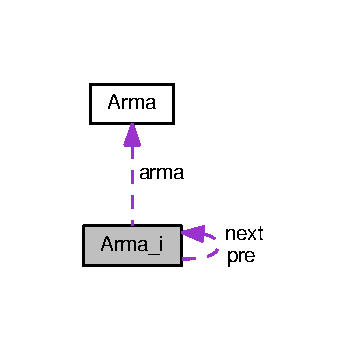
\includegraphics[width=167pt]{structArma__i__coll__graph}
\end{center}
\end{figure}
\subsection*{Public Attributes}
\begin{DoxyCompactItemize}
\item 
\hypertarget{structArma__i_a31995f30ab4fa1c15bf90dd36f005e65}{}\hyperlink{classArma}{Arma} $\ast$ \hyperlink{structArma__i_a31995f30ab4fa1c15bf90dd36f005e65}{arma}\label{structArma__i_a31995f30ab4fa1c15bf90dd36f005e65}

\begin{DoxyCompactList}\small\item\em puntatore ad arma \end{DoxyCompactList}\item 
\hypertarget{structArma__i_a5c7efd2cb17b565aabc418d81ce38041}{}char \hyperlink{structArma__i_a5c7efd2cb17b565aabc418d81ce38041}{draw} \mbox{[}25\mbox{]}\mbox{[}79\mbox{]}\label{structArma__i_a5c7efd2cb17b565aabc418d81ce38041}

\begin{DoxyCompactList}\small\item\em matrice della picture \end{DoxyCompactList}\item 
\hypertarget{structArma__i_aa998dac5a34bbb1afb58fcc3c7c196ab}{}\hyperlink{structArma__i}{Arma\+\_\+i} $\ast$ \hyperlink{structArma__i_aa998dac5a34bbb1afb58fcc3c7c196ab}{next}\label{structArma__i_aa998dac5a34bbb1afb58fcc3c7c196ab}

\begin{DoxyCompactList}\small\item\em puntatore al nodo succesivo \end{DoxyCompactList}\item 
\hypertarget{structArma__i_ac43ce4b132cbb5f75ec895ea1806d0ee}{}\hyperlink{structArma__i}{Arma\+\_\+i} $\ast$ \hyperlink{structArma__i_ac43ce4b132cbb5f75ec895ea1806d0ee}{pre}\label{structArma__i_ac43ce4b132cbb5f75ec895ea1806d0ee}

\begin{DoxyCompactList}\small\item\em puntatore al nodo precedente \end{DoxyCompactList}\end{DoxyCompactItemize}


\subsection{Detailed Description}
Questa struct definisce una lista bidirezionale di armi con la rispettiva picture. 

The documentation for this struct was generated from the following file\+:\begin{DoxyCompactItemize}
\item 
\hyperlink{Animazioni_8hpp}{Animazioni.\+hpp}\end{DoxyCompactItemize}

\hypertarget{structcollisione}{}\section{collisione Struct Reference}
\label{structcollisione}\index{collisione@{collisione}}


Questa struct definisce una collisione tra un\textquotesingle{}entità ed un proiettile.  




{\ttfamily \#include $<$Structure.\+hpp$>$}



Collaboration diagram for collisione\+:\nopagebreak
\begin{figure}[H]
\begin{center}
\leavevmode
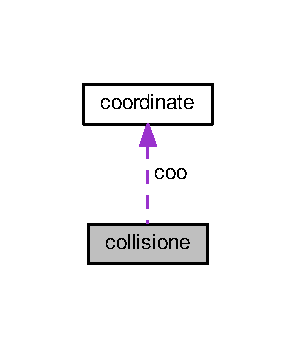
\includegraphics[width=142pt]{structcollisione__coll__graph}
\end{center}
\end{figure}
\subsection*{Public Attributes}
\begin{DoxyCompactItemize}
\item 
\hypertarget{structcollisione_aaf479a890eeb967854b96931cb517dbe}{}\hyperlink{structcoordinate}{coordinate} \hyperlink{structcollisione_aaf479a890eeb967854b96931cb517dbe}{coo}\label{structcollisione_aaf479a890eeb967854b96931cb517dbe}

\begin{DoxyCompactList}\small\item\em coordinate dell\textquotesingle{}entita collisa \end{DoxyCompactList}\item 
\hypertarget{structcollisione_adb4901ff23217f71261e39108936b612}{}char \hyperlink{structcollisione_adb4901ff23217f71261e39108936b612}{chi}\label{structcollisione_adb4901ff23217f71261e39108936b612}

\begin{DoxyCompactList}\small\item\em carattere dell\textquotesingle{}entita collisa \end{DoxyCompactList}\item 
\hypertarget{structcollisione_a473c8f33976fa65d868b0b19c44001d3}{}int \hyperlink{structcollisione_a473c8f33976fa65d868b0b19c44001d3}{volte}\label{structcollisione_a473c8f33976fa65d868b0b19c44001d3}

\begin{DoxyCompactList}\small\item\em quante volta l\textquotesingle{}entità è stata colpita \end{DoxyCompactList}\item 
\hypertarget{structcollisione_a3d7c2d8bc4438556813228157d31f812}{}int {\bfseries danno}\label{structcollisione_a3d7c2d8bc4438556813228157d31f812}

\end{DoxyCompactItemize}


\subsection{Detailed Description}
Questa struct definisce una collisione tra un\textquotesingle{}entità ed un proiettile. 

The documentation for this struct was generated from the following file\+:\begin{DoxyCompactItemize}
\item 
Structure.\+hpp\end{DoxyCompactItemize}

\input{structController}
\hypertarget{structcontroller}{}\section{controller Struct Reference}
\label{structcontroller}\index{controller@{controller}}


Questa struct definisce i comandi che l\textquotesingle{}untente può impartire al gioco.  




{\ttfamily \#include $<$Structure.\+hpp$>$}



\subsection{Detailed Description}
Questa struct definisce i comandi che l\textquotesingle{}untente può impartire al gioco. 

The documentation for this struct was generated from the following file\+:\begin{DoxyCompactItemize}
\item 
Structure.\+hpp\end{DoxyCompactItemize}

\hypertarget{structcoordinate}{}\section{coordinate Struct Reference}
\label{structcoordinate}\index{coordinate@{coordinate}}


Questa struct definisce le coordinate riferite localmente all stanza.  




{\ttfamily \#include $<$Structure.\+hpp$>$}

\subsection*{Public Attributes}
\begin{DoxyCompactItemize}
\item 
\hypertarget{structcoordinate_a1431128cf99def93975d05db27bc251f}{}int \hyperlink{structcoordinate_a1431128cf99def93975d05db27bc251f}{x}\label{structcoordinate_a1431128cf99def93975d05db27bc251f}

\begin{DoxyCompactList}\small\item\em ascissa \end{DoxyCompactList}\item 
\hypertarget{structcoordinate_aee8f883e3734f5c1e4be9425c7308a35}{}int \hyperlink{structcoordinate_aee8f883e3734f5c1e4be9425c7308a35}{y}\label{structcoordinate_aee8f883e3734f5c1e4be9425c7308a35}

\begin{DoxyCompactList}\small\item\em ordinata \end{DoxyCompactList}\end{DoxyCompactItemize}


\subsection{Detailed Description}
Questa struct definisce le coordinate riferite localmente all stanza. 

The documentation for this struct was generated from the following file\+:\begin{DoxyCompactItemize}
\item 
Structure.\+hpp\end{DoxyCompactItemize}

\hypertarget{classGame}{}\section{Game Class Reference}
\label{classGame}\index{Game@{Game}}
\subsection*{Public Member Functions}
\begin{DoxyCompactItemize}
\item 
\hypertarget{classGame_aae5e55d577a93b1f8428c7e3da67556b}{}{\bfseries Game} (\hyperlink{classGiocatore}{Giocatore} $\ast$gamer)\label{classGame_aae5e55d577a93b1f8428c7e3da67556b}

\item 
\hypertarget{classGame_abdfaff95e8b4c780a2354f5e43791c50}{}\hyperlink{structController}{Controller} $\ast$ {\bfseries get\+Controller} ()\label{classGame_abdfaff95e8b4c780a2354f5e43791c50}

\item 
\hypertarget{classGame_aa7f7f85608835ceea8720d798e483dee}{}\hyperlink{classAnimazioni}{Animazioni} $\ast$ {\bfseries get\+Animazioni} ()\label{classGame_aa7f7f85608835ceea8720d798e483dee}

\item 
\hypertarget{classGame_ad640d42e1d6a92ba8d0da9aa3aca941f}{}void {\bfseries draw\+\_\+details} ()\label{classGame_ad640d42e1d6a92ba8d0da9aa3aca941f}

\item 
\hypertarget{classGame_a06fb0be2666888d7ff35fa5793d29867}{}void {\bfseries aggiorna\+\_\+turni} ()\label{classGame_a06fb0be2666888d7ff35fa5793d29867}

\item 
\hypertarget{classGame_a3d9b98f7c4a96ecf578f75b96c9f0e90}{}void {\bfseries start} ()\label{classGame_a3d9b98f7c4a96ecf578f75b96c9f0e90}

\end{DoxyCompactItemize}


The documentation for this class was generated from the following files\+:\begin{DoxyCompactItemize}
\item 
Game.\+hpp\item 
Game.\+cpp\end{DoxyCompactItemize}

\hypertarget{classGiocatore}{}\section{Giocatore Class Reference}
\label{classGiocatore}\index{Giocatore@{Giocatore}}


Figlia di \hyperlink{classPersona}{Persona} definisce le specifiche aggiuntive del giocatore utente.  




{\ttfamily \#include $<$Giocatore.\+hpp$>$}



Inheritance diagram for Giocatore\+:\nopagebreak
\begin{figure}[H]
\begin{center}
\leavevmode
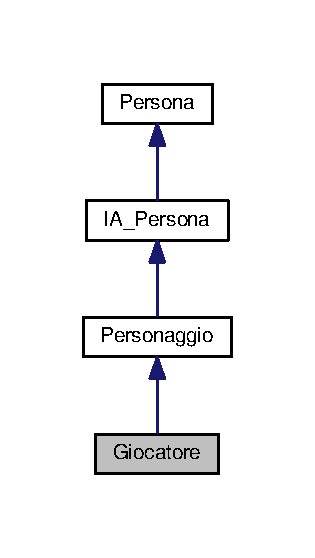
\includegraphics[width=151pt]{classGiocatore__inherit__graph}
\end{center}
\end{figure}


Collaboration diagram for Giocatore\+:\nopagebreak
\begin{figure}[H]
\begin{center}
\leavevmode
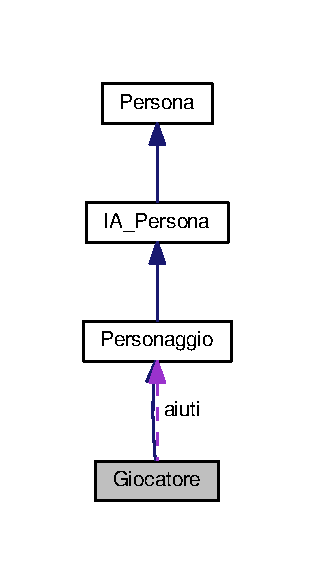
\includegraphics[width=151pt]{classGiocatore__coll__graph}
\end{center}
\end{figure}
\subsection*{Public Member Functions}
\begin{DoxyCompactItemize}
\item 
\hyperlink{classGiocatore_ab05bd16f9ab3323dc827c1cb41bf185e}{Giocatore} (char \hyperlink{classPersona_a15d4ded972e8bdd3f02e89c6ccb71b73}{nome}\mbox{[}$\,$\mbox{]}, char \hyperlink{classPersona_ae7069f0467a3b2f1d269c1a143b730eb}{tipo}\mbox{[}$\,$\mbox{]}, int \hyperlink{classPersona_a1e784d3a56cddd6ba8e81387df1efc7b}{vita}, char \hyperlink{classPersona_a1fff44e46be477b79413387307b0aaff}{carattere})
\begin{DoxyCompactList}\small\item\em Costruttore. \end{DoxyCompactList}\item 
int \hyperlink{classGiocatore_a1f05e45f9694771260a7f9aee5265821}{add\+Aiutante} (\hyperlink{classPersonaggio}{Personaggio} nuovo)
\begin{DoxyCompactList}\small\item\em aggiunge un nuovo aiutante nel vettore aiuti (=0 se ha aggiunto nuovo, !=0 altrimenti) \end{DoxyCompactList}\item 
bool \hyperlink{classGiocatore_a703b38cbe7f7657ff98018878c15a961}{remove\+Aiutante} (\hyperlink{classPersonaggio}{Personaggio} aiuto)
\begin{DoxyCompactList}\small\item\em rimuove aiutante aiuto dal vettore aiuti (true se ha eliminato aiuto, false altrimenti) \end{DoxyCompactList}\item 
bool \hyperlink{classGiocatore_ac9f5c0e981bddc91a6b93b4a6fa48e46}{replace\+Aiutante} (\hyperlink{classPersonaggio}{Personaggio} old, \hyperlink{classPersonaggio}{Personaggio} nuovo)
\begin{DoxyCompactList}\small\item\em sostituisce l\textquotesingle{}aiutante old con quello buovo nel vettore aiuti (true se ha sostituito, false altrimenti) \end{DoxyCompactList}\item 
int \hyperlink{classGiocatore_a6ed5fb81af05df594102a6f6d5d7cbd9}{get\+Index\+Aiutante} (\hyperlink{classPersonaggio}{Personaggio} aiuto)
\begin{DoxyCompactList}\small\item\em ritorna l\textquotesingle{}indice dl vettore riferito ad aiuto \end{DoxyCompactList}\item 
\hypertarget{classGiocatore_afd1c7f8a65c41d78c245782459fede3f}{}int \hyperlink{classGiocatore_afd1c7f8a65c41d78c245782459fede3f}{get\+Num\+Aiutanti} ()\label{classGiocatore_afd1c7f8a65c41d78c245782459fede3f}

\begin{DoxyCompactList}\small\item\em ritorna il numero di aiutanti attualmente presenti nel vettore di aiuti \end{DoxyCompactList}\item 
bool \hyperlink{classGiocatore_acb3e7fc5a268671fb5d2628610a91040}{compare\+Persona} (\hyperlink{classPersonaggio}{Personaggio} p, int i)
\begin{DoxyCompactList}\small\item\em confronta l\textquotesingle{}aiutante p con quello presente nella posizione i-\/esima del vettore di aiuti \end{DoxyCompactList}\end{DoxyCompactItemize}
\subsection*{Public Attributes}
\begin{DoxyCompactItemize}
\item 
\hypertarget{classGiocatore_a051497cae381d27b07def9e89231bf6d}{}\hyperlink{classPersonaggio}{Personaggio} $\ast$ \hyperlink{classGiocatore_a051497cae381d27b07def9e89231bf6d}{aiuti} \mbox{[}\hyperlink{classGiocatore_afb448871b667ab644a2a32a0ade42e39}{num\+\_\+max\+\_\+aiuti}\mbox{]}\label{classGiocatore_a051497cae381d27b07def9e89231bf6d}

\begin{DoxyCompactList}\small\item\em vettore degli aiutanti \end{DoxyCompactList}\item 
\hypertarget{classGiocatore_a8c7c227c90ed564f4e370c790cbef97d}{}int \hyperlink{classGiocatore_a8c7c227c90ed564f4e370c790cbef97d}{num\+\_\+aiuti}\label{classGiocatore_a8c7c227c90ed564f4e370c790cbef97d}

\begin{DoxyCompactList}\small\item\em numero di aiutanti attualmente presenti nel vettore aiuti \end{DoxyCompactList}\end{DoxyCompactItemize}
\subsection*{Static Public Attributes}
\begin{DoxyCompactItemize}
\item 
\hypertarget{classGiocatore_afb448871b667ab644a2a32a0ade42e39}{}static const int \hyperlink{classGiocatore_afb448871b667ab644a2a32a0ade42e39}{num\+\_\+max\+\_\+aiuti} =5\label{classGiocatore_afb448871b667ab644a2a32a0ade42e39}

\begin{DoxyCompactList}\small\item\em costante che indica il numero massimo di aiutanti che si possono avere \end{DoxyCompactList}\end{DoxyCompactItemize}
\subsection*{Additional Inherited Members}


\subsection{Detailed Description}
Figlia di \hyperlink{classPersona}{Persona} definisce le specifiche aggiuntive del giocatore utente. 

\subsection{Constructor \& Destructor Documentation}
\hypertarget{classGiocatore_ab05bd16f9ab3323dc827c1cb41bf185e}{}\index{Giocatore@{Giocatore}!Giocatore@{Giocatore}}
\index{Giocatore@{Giocatore}!Giocatore@{Giocatore}}
\subsubsection[{Giocatore}]{\setlength{\rightskip}{0pt plus 5cm}Giocatore\+::\+Giocatore (
\begin{DoxyParamCaption}
\item[{char}]{nome\mbox{[}$\,$\mbox{]}, }
\item[{char}]{tipo\mbox{[}$\,$\mbox{]}, }
\item[{int}]{vita, }
\item[{char}]{carattere}
\end{DoxyParamCaption}
)}\label{classGiocatore_ab05bd16f9ab3323dc827c1cb41bf185e}


Costruttore. 


\begin{DoxyParams}{Parameters}
{\em nome} & nome della persona \\
\hline
{\em tipo} & tipo della persona \\
\hline
{\em vita} & unità di vita della persona \\
\hline
{\em carattere} & carattere stampato a video della persona \\
\hline
\end{DoxyParams}


\subsection{Member Function Documentation}
\hypertarget{classGiocatore_a1f05e45f9694771260a7f9aee5265821}{}\index{Giocatore@{Giocatore}!add\+Aiutante@{add\+Aiutante}}
\index{add\+Aiutante@{add\+Aiutante}!Giocatore@{Giocatore}}
\subsubsection[{add\+Aiutante}]{\setlength{\rightskip}{0pt plus 5cm}Giocatore\+::add\+Aiutante (
\begin{DoxyParamCaption}
\item[{{\bf Personaggio}}]{nuovo}
\end{DoxyParamCaption}
)}\label{classGiocatore_a1f05e45f9694771260a7f9aee5265821}


aggiunge un nuovo aiutante nel vettore aiuti (=0 se ha aggiunto nuovo, !=0 altrimenti) 


\begin{DoxyParams}{Parameters}
{\em nuovo} & nuovo aiutante da inserire \\
\hline
\end{DoxyParams}
\hypertarget{classGiocatore_acb3e7fc5a268671fb5d2628610a91040}{}\index{Giocatore@{Giocatore}!compare\+Persona@{compare\+Persona}}
\index{compare\+Persona@{compare\+Persona}!Giocatore@{Giocatore}}
\subsubsection[{compare\+Persona}]{\setlength{\rightskip}{0pt plus 5cm}Giocatore\+::compare\+Persona (
\begin{DoxyParamCaption}
\item[{{\bf Personaggio}}]{p, }
\item[{int}]{i}
\end{DoxyParamCaption}
)}\label{classGiocatore_acb3e7fc5a268671fb5d2628610a91040}


confronta l\textquotesingle{}aiutante p con quello presente nella posizione i-\/esima del vettore di aiuti 


\begin{DoxyParams}{Parameters}
{\em p} & aiutante da confrontare \\
\hline
{\em i} & indice del secondo aiutante da confrontare \\
\hline
\end{DoxyParams}
\hypertarget{classGiocatore_a6ed5fb81af05df594102a6f6d5d7cbd9}{}\index{Giocatore@{Giocatore}!get\+Index\+Aiutante@{get\+Index\+Aiutante}}
\index{get\+Index\+Aiutante@{get\+Index\+Aiutante}!Giocatore@{Giocatore}}
\subsubsection[{get\+Index\+Aiutante}]{\setlength{\rightskip}{0pt plus 5cm}Giocatore\+::get\+Index\+Aiutante (
\begin{DoxyParamCaption}
\item[{{\bf Personaggio}}]{aiuto}
\end{DoxyParamCaption}
)}\label{classGiocatore_a6ed5fb81af05df594102a6f6d5d7cbd9}


ritorna l\textquotesingle{}indice dl vettore riferito ad aiuto 


\begin{DoxyParams}{Parameters}
{\em aiuto} & aiutante che si vuole conoscere il suo indice \\
\hline
\end{DoxyParams}
\hypertarget{classGiocatore_a703b38cbe7f7657ff98018878c15a961}{}\index{Giocatore@{Giocatore}!remove\+Aiutante@{remove\+Aiutante}}
\index{remove\+Aiutante@{remove\+Aiutante}!Giocatore@{Giocatore}}
\subsubsection[{remove\+Aiutante}]{\setlength{\rightskip}{0pt plus 5cm}Giocatore\+::remove\+Aiutante (
\begin{DoxyParamCaption}
\item[{{\bf Personaggio}}]{aiuto}
\end{DoxyParamCaption}
)}\label{classGiocatore_a703b38cbe7f7657ff98018878c15a961}


rimuove aiutante aiuto dal vettore aiuti (true se ha eliminato aiuto, false altrimenti) 


\begin{DoxyParams}{Parameters}
{\em aiuto} & aiutante da rimuovere \\
\hline
\end{DoxyParams}
\hypertarget{classGiocatore_ac9f5c0e981bddc91a6b93b4a6fa48e46}{}\index{Giocatore@{Giocatore}!replace\+Aiutante@{replace\+Aiutante}}
\index{replace\+Aiutante@{replace\+Aiutante}!Giocatore@{Giocatore}}
\subsubsection[{replace\+Aiutante}]{\setlength{\rightskip}{0pt plus 5cm}Giocatore\+::replace\+Aiutante (
\begin{DoxyParamCaption}
\item[{{\bf Personaggio}}]{old, }
\item[{{\bf Personaggio}}]{nuovo}
\end{DoxyParamCaption}
)}\label{classGiocatore_ac9f5c0e981bddc91a6b93b4a6fa48e46}


sostituisce l\textquotesingle{}aiutante old con quello buovo nel vettore aiuti (true se ha sostituito, false altrimenti) 


\begin{DoxyParams}{Parameters}
{\em old} & aiutante da sostituire \\
\hline
{\em nuovo} & nuovo aiutante \\
\hline
\end{DoxyParams}


The documentation for this class was generated from the following files\+:\begin{DoxyCompactItemize}
\item 
\hyperlink{Giocatore_8hpp}{Giocatore.\+hpp}\item 
Giocatore.\+cpp\end{DoxyCompactItemize}

\hypertarget{classIA__Persona}{}\section{I\+A\+\_\+\+Persona Class Reference}
\label{classIA__Persona}\index{I\+A\+\_\+\+Persona@{I\+A\+\_\+\+Persona}}


Gestisce tutte le azioni che vengono considerate come azioni del turno di gioco.  




{\ttfamily \#include $<$I\+A\+\_\+\+Persona.\+hpp$>$}



Inheritance diagram for I\+A\+\_\+\+Persona\+:\nopagebreak
\begin{figure}[H]
\begin{center}
\leavevmode
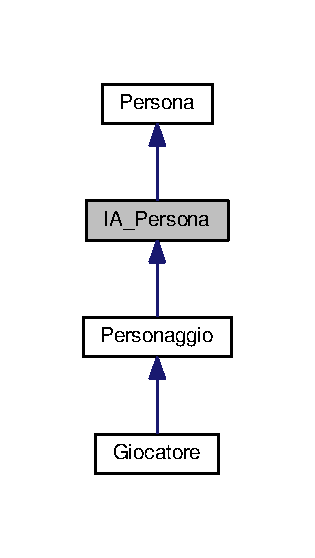
\includegraphics[width=151pt]{classIA__Persona__inherit__graph}
\end{center}
\end{figure}


Collaboration diagram for I\+A\+\_\+\+Persona\+:\nopagebreak
\begin{figure}[H]
\begin{center}
\leavevmode
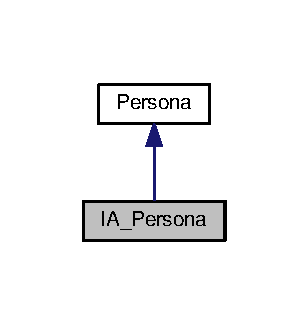
\includegraphics[width=148pt]{classIA__Persona__coll__graph}
\end{center}
\end{figure}
\subsection*{Public Member Functions}
\begin{DoxyCompactItemize}
\item 
\hyperlink{classIA__Persona_a450a8b02b473b9bc110d65a47326a069}{I\+A\+\_\+\+Persona} (char \hyperlink{classPersona_a15d4ded972e8bdd3f02e89c6ccb71b73}{nome}\mbox{[}50\mbox{]}, char \hyperlink{classPersona_ae7069f0467a3b2f1d269c1a143b730eb}{tipo}\mbox{[}50\mbox{]}, char \hyperlink{classPersona_a1fff44e46be477b79413387307b0aaff}{carattere}, int \hyperlink{classPersona_a1e784d3a56cddd6ba8e81387df1efc7b}{vita})
\begin{DoxyCompactList}\small\item\em Costruttore. \end{DoxyCompactList}\item 
void \hyperlink{classIA__Persona_ab8820ce00b02a098bf917e53bf297051}{write\+\_\+object} (char stanza\mbox{[}25\mbox{]}\mbox{[}91\mbox{]}, \hyperlink{structOggetto__pos}{Oggetto\+\_\+pos} $\ast$$\ast$raccogliere, int num\+\_\+oggetti)
\begin{DoxyCompactList}\small\item\em stampa sulla matrice della stanza tutti gli oggetti raccoglibili \end{DoxyCompactList}\item 
\hypertarget{classIA__Persona_a33a4375ebb8e374fd92c88759e28e492}{}bool \hyperlink{classIA__Persona_a33a4375ebb8e374fd92c88759e28e492}{get\+Scudo} ()\label{classIA__Persona_a33a4375ebb8e374fd92c88759e28e492}

\begin{DoxyCompactList}\small\item\em Ritorna lo stato dello scudo. \end{DoxyCompactList}\item 
bool \hyperlink{classIA__Persona_a71520669c85eea90e2fd1dac2a7372d0}{set\+Scudo} (bool \hyperlink{classPersona_a1af99e040deeb7015e7e99bb2a5128f4}{scudo})
\begin{DoxyCompactList}\small\item\em Modifica lo stato dello scudo. \end{DoxyCompactList}\item 
bool \hyperlink{classIA__Persona_aad9235e41742654f77ea0abc771e51c4}{passo} (\hyperlink{structController}{Controller} $\ast$\hyperlink{structcontroller}{controller}, \hyperlink{structcoordinate}{coordinate} $\ast$new\+\_\+coordinate, char direction, char stanza\mbox{[}25\mbox{]}\mbox{[}91\mbox{]})
\begin{DoxyCompactList}\small\item\em effettua l\textquotesingle{}avazamento sulla stanza della persona \end{DoxyCompactList}\item 
bool \hyperlink{classIA__Persona_ad8ad21a6a106d3d98e18d1c33f906f87}{raccogli} (\hyperlink{structController}{Controller} $\ast$\hyperlink{structcontroller}{controller}, char direction, char stanza\mbox{[}25\mbox{]}\mbox{[}91\mbox{]}, \hyperlink{structcoordinate}{coordinate} coo\+\_\+stanza, \hyperlink{structOggetto__pos}{Oggetto\+\_\+pos} $\ast$$\ast$raccogliere, int num\+\_\+oggetti, int $\ast$total\+\_\+time\+\_\+machine\+\_\+part\+\_\+catched, int local\+\_\+time\+\_\+machine\+\_\+part, \hyperlink{structTime__Machine}{Time\+\_\+\+Machine} $\ast$$\ast$time\+\_\+machine\+\_\+coo)
\begin{DoxyCompactList}\small\item\em effettua l\textquotesingle{}avazamento sulla stanza della persona \end{DoxyCompactList}\item 
bool \hyperlink{classIA__Persona_abd04c4e981f7e1260784c1d7f7a3614f}{spara} (\hyperlink{structController}{Controller} $\ast$\hyperlink{structcontroller}{controller}, char direction, char stanza\mbox{[}25\mbox{]}\mbox{[}91\mbox{]}, \hyperlink{structcoordinate}{coordinate} coo\+\_\+stanza, \hyperlink{classPersona}{Persona} $\ast$persone\mbox{[}$\,$\mbox{]}, int num\+\_\+persone)
\begin{DoxyCompactList}\small\item\em effettua l\textquotesingle{}avazamento sulla stanza della persona \end{DoxyCompactList}\item 
void \hyperlink{classIA__Persona_a361953a09f5d4b94f29824e2f1b83c15}{dialoga} (\hyperlink{classPersona}{Persona} $\ast$giocatore, \hyperlink{classPersona}{Persona} $\ast$persone\mbox{[}$\,$\mbox{]}, int num\+\_\+persone, \hyperlink{structController}{Controller} $\ast$\hyperlink{structcontroller}{controller}, char direction, char stanza\mbox{[}25\mbox{]}\mbox{[}91\mbox{]}, \hyperlink{structcoordinate}{coordinate} diallogo\+\_\+coo, int livello)
\begin{DoxyCompactList}\small\item\em effettua l\textquotesingle{}avazamento sulla stanza della persona \end{DoxyCompactList}\end{DoxyCompactItemize}
\subsection*{Additional Inherited Members}


\subsection{Detailed Description}
Gestisce tutte le azioni che vengono considerate come azioni del turno di gioco. 

\subsection{Constructor \& Destructor Documentation}
\hypertarget{classIA__Persona_a450a8b02b473b9bc110d65a47326a069}{}\index{I\+A\+\_\+\+Persona@{I\+A\+\_\+\+Persona}!I\+A\+\_\+\+Persona@{I\+A\+\_\+\+Persona}}
\index{I\+A\+\_\+\+Persona@{I\+A\+\_\+\+Persona}!I\+A\+\_\+\+Persona@{I\+A\+\_\+\+Persona}}
\subsubsection[{I\+A\+\_\+\+Persona}]{\setlength{\rightskip}{0pt plus 5cm}I\+A\+\_\+\+Persona\+::\+I\+A\+\_\+\+Persona (
\begin{DoxyParamCaption}
\item[{char}]{nome\mbox{[}50\mbox{]}, }
\item[{char}]{tipo\mbox{[}50\mbox{]}, }
\item[{char}]{carattere, }
\item[{int}]{vita}
\end{DoxyParamCaption}
)}\label{classIA__Persona_a450a8b02b473b9bc110d65a47326a069}


Costruttore. 


\begin{DoxyParams}{Parameters}
{\em nome\mbox{[}$\,$\mbox{]}} & nome della persona \\
\hline
{\em tipo\mbox{[}$\,$\mbox{]}} & tipo della persona \\
\hline
{\em carattere} & carattere della persona \\
\hline
{\em vita} & vita della persona \\
\hline
\end{DoxyParams}


\subsection{Member Function Documentation}
\hypertarget{classIA__Persona_a361953a09f5d4b94f29824e2f1b83c15}{}\index{I\+A\+\_\+\+Persona@{I\+A\+\_\+\+Persona}!dialoga@{dialoga}}
\index{dialoga@{dialoga}!I\+A\+\_\+\+Persona@{I\+A\+\_\+\+Persona}}
\subsubsection[{dialoga}]{\setlength{\rightskip}{0pt plus 5cm}I\+A\+\_\+\+Persona\+::dialoga (
\begin{DoxyParamCaption}
\item[{{\bf Persona} $\ast$}]{giocatore, }
\item[{{\bf Persona} $\ast$}]{persone\mbox{[}$\,$\mbox{]}, }
\item[{int}]{num\+\_\+persone, }
\item[{{\bf Controller} $\ast$}]{controller, }
\item[{char}]{direction, }
\item[{char}]{stanza\mbox{[}25\mbox{]}\mbox{[}91\mbox{]}, }
\item[{{\bf coordinate}}]{diallogo\+\_\+coo, }
\item[{int}]{livello}
\end{DoxyParamCaption}
)}\label{classIA__Persona_a361953a09f5d4b94f29824e2f1b83c15}


effettua l\textquotesingle{}avazamento sulla stanza della persona 


\begin{DoxyParams}{Parameters}
{\em giocatore} & puntatore al giocatore \\
\hline
{\em persone\mbox{[}$\,$\mbox{]}} & tutte le persone presenti nella (fatta eccezione per i nemici) con cui è possibile dialogare \\
\hline
{\em num\+\_\+persone} & numero di persone presenti nella (fatta eccezione per i nemici) con cui è possibile dialogare \\
\hline
{\em controller} & puntatore all\textquotesingle{}instanza di tipo \hyperlink{structController}{Controller} per l\textquotesingle{}insieme di tutti i comandi utente \\
\hline
{\em direction} & direzione in cui la persona deve andare definito dal controller \\
\hline
{\em stanza\mbox{[}$\,$\mbox{]}\mbox{[}$\,$\mbox{]}} & matrice della stanza \\
\hline
{\em diallogo\+\_\+coo} & coordinate della messa a video del dialogo \\
\hline
{\em livello} & numero del livello durante il dialogo \\
\hline
\end{DoxyParams}
\hypertarget{classIA__Persona_aad9235e41742654f77ea0abc771e51c4}{}\index{I\+A\+\_\+\+Persona@{I\+A\+\_\+\+Persona}!passo@{passo}}
\index{passo@{passo}!I\+A\+\_\+\+Persona@{I\+A\+\_\+\+Persona}}
\subsubsection[{passo}]{\setlength{\rightskip}{0pt plus 5cm}I\+A\+\_\+\+Persona\+::passo (
\begin{DoxyParamCaption}
\item[{{\bf Controller} $\ast$}]{controller, }
\item[{{\bf coordinate} $\ast$}]{new\+\_\+coordinate, }
\item[{char}]{direction, }
\item[{char}]{stanza\mbox{[}25\mbox{]}\mbox{[}91\mbox{]}}
\end{DoxyParamCaption}
)}\label{classIA__Persona_aad9235e41742654f77ea0abc771e51c4}


effettua l\textquotesingle{}avazamento sulla stanza della persona 


\begin{DoxyParams}{Parameters}
{\em controller} & puntatore all\textquotesingle{}instanza di tipo \hyperlink{structController}{Controller} per l\textquotesingle{}insieme di tutti i comandi utente \\
\hline
{\em new\+\_\+coordinate} & possibilita di avere le coordinate aggiornate \mbox{[}Opzionale\mbox{]} \\
\hline
{\em direction} & direzione in cui la persona deve andare definito dal controller \\
\hline
{\em stanza\mbox{[}$\,$\mbox{]}\mbox{[}$\,$\mbox{]}} & matrice della stanza \\
\hline
\end{DoxyParams}
\hypertarget{classIA__Persona_ad8ad21a6a106d3d98e18d1c33f906f87}{}\index{I\+A\+\_\+\+Persona@{I\+A\+\_\+\+Persona}!raccogli@{raccogli}}
\index{raccogli@{raccogli}!I\+A\+\_\+\+Persona@{I\+A\+\_\+\+Persona}}
\subsubsection[{raccogli}]{\setlength{\rightskip}{0pt plus 5cm}I\+A\+\_\+\+Persona\+::raccogli (
\begin{DoxyParamCaption}
\item[{{\bf Controller} $\ast$}]{controller, }
\item[{char}]{direction, }
\item[{char}]{stanza\mbox{[}25\mbox{]}\mbox{[}91\mbox{]}, }
\item[{{\bf coordinate}}]{coo\+\_\+stanza, }
\item[{{\bf Oggetto\+\_\+pos} $\ast$$\ast$}]{raccogliere, }
\item[{int}]{num\+\_\+oggetti, }
\item[{int $\ast$}]{total\+\_\+time\+\_\+machine\+\_\+part\+\_\+catched, }
\item[{int}]{local\+\_\+time\+\_\+machine\+\_\+part, }
\item[{{\bf Time\+\_\+\+Machine} $\ast$$\ast$}]{time\+\_\+machine\+\_\+coo}
\end{DoxyParamCaption}
)}\label{classIA__Persona_ad8ad21a6a106d3d98e18d1c33f906f87}


effettua l\textquotesingle{}avazamento sulla stanza della persona 


\begin{DoxyParams}{Parameters}
{\em controller} & puntatore all\textquotesingle{}instanza di tipo \hyperlink{structController}{Controller} per l\textquotesingle{}insieme di tutti i comandi utente \\
\hline
{\em direction} & direzione in cui la persona deve andare definito dal controller \\
\hline
{\em stanza\mbox{[}$\,$\mbox{]}\mbox{[}$\,$\mbox{]}} & matrice della stanza \\
\hline
{\em coo\+\_\+stanza} & coordinate della stanza sullo schermo \\
\hline
{\em raccogliere} & oggetti raccoglibili della stanza \\
\hline
{\em num\+\_\+oggetti} & numero di oggetti raccoglibili \\
\hline
\end{DoxyParams}
\hypertarget{classIA__Persona_a71520669c85eea90e2fd1dac2a7372d0}{}\index{I\+A\+\_\+\+Persona@{I\+A\+\_\+\+Persona}!set\+Scudo@{set\+Scudo}}
\index{set\+Scudo@{set\+Scudo}!I\+A\+\_\+\+Persona@{I\+A\+\_\+\+Persona}}
\subsubsection[{set\+Scudo}]{\setlength{\rightskip}{0pt plus 5cm}I\+A\+\_\+\+Persona\+::set\+Scudo (
\begin{DoxyParamCaption}
\item[{bool}]{scudo}
\end{DoxyParamCaption}
)}\label{classIA__Persona_a71520669c85eea90e2fd1dac2a7372d0}


Modifica lo stato dello scudo. 


\begin{DoxyParams}{Parameters}
{\em scudo} & nuovo stato dello scudo \\
\hline
\end{DoxyParams}
\hypertarget{classIA__Persona_abd04c4e981f7e1260784c1d7f7a3614f}{}\index{I\+A\+\_\+\+Persona@{I\+A\+\_\+\+Persona}!spara@{spara}}
\index{spara@{spara}!I\+A\+\_\+\+Persona@{I\+A\+\_\+\+Persona}}
\subsubsection[{spara}]{\setlength{\rightskip}{0pt plus 5cm}I\+A\+\_\+\+Persona\+::spara (
\begin{DoxyParamCaption}
\item[{{\bf Controller} $\ast$}]{controller, }
\item[{char}]{direction, }
\item[{char}]{stanza\mbox{[}25\mbox{]}\mbox{[}91\mbox{]}, }
\item[{{\bf coordinate}}]{coo\+\_\+stanza, }
\item[{{\bf Persona} $\ast$}]{persone\mbox{[}$\,$\mbox{]}, }
\item[{int}]{num\+\_\+persone}
\end{DoxyParamCaption}
)}\label{classIA__Persona_abd04c4e981f7e1260784c1d7f7a3614f}


effettua l\textquotesingle{}avazamento sulla stanza della persona 


\begin{DoxyParams}{Parameters}
{\em controller} & puntatore all\textquotesingle{}instanza di tipo \hyperlink{structController}{Controller} per l\textquotesingle{}insieme di tutti i comandi utente \\
\hline
{\em direction} & direzione in cui la persona deve andare definito dal controller \\
\hline
{\em stanza\mbox{[}$\,$\mbox{]}\mbox{[}$\,$\mbox{]}} & matrice della stanza \\
\hline
{\em coo\+\_\+stanza} & coordinate della stanza sullo schermo \\
\hline
{\em persone\mbox{[}$\,$\mbox{]}} & vettore di tutte le persone presenti nella stanza \\
\hline
{\em num\+\_\+persone} & numero di persone presenti nella stanza \\
\hline
\end{DoxyParams}
\hypertarget{classIA__Persona_ab8820ce00b02a098bf917e53bf297051}{}\index{I\+A\+\_\+\+Persona@{I\+A\+\_\+\+Persona}!write\+\_\+object@{write\+\_\+object}}
\index{write\+\_\+object@{write\+\_\+object}!I\+A\+\_\+\+Persona@{I\+A\+\_\+\+Persona}}
\subsubsection[{write\+\_\+object}]{\setlength{\rightskip}{0pt plus 5cm}I\+A\+\_\+\+Persona\+::write\+\_\+object (
\begin{DoxyParamCaption}
\item[{char}]{stanza\mbox{[}25\mbox{]}\mbox{[}91\mbox{]}, }
\item[{{\bf Oggetto\+\_\+pos} $\ast$$\ast$}]{raccogliere, }
\item[{int}]{num\+\_\+oggetti}
\end{DoxyParamCaption}
)}\label{classIA__Persona_ab8820ce00b02a098bf917e53bf297051}


stampa sulla matrice della stanza tutti gli oggetti raccoglibili 


\begin{DoxyParams}{Parameters}
{\em stanza\mbox{[}$\,$\mbox{]}\mbox{[}$\,$\mbox{]}} & matrice della stanza \\
\hline
{\em raccogliere} & vettore di oggetti che si possono raccogliere \\
\hline
{\em num\+\_\+oggetti} & numero di oggetti che si possono raccogliere \\
\hline
\end{DoxyParams}


The documentation for this class was generated from the following files\+:\begin{DoxyCompactItemize}
\item 
\hyperlink{IA__Persona_8hpp}{I\+A\+\_\+\+Persona.\+hpp}\item 
I\+A\+\_\+\+Persona.\+cpp\end{DoxyCompactItemize}

\hypertarget{structKIT}{}\section{K\+I\+T Struct Reference}
\label{structKIT}\index{K\+I\+T@{K\+I\+T}}


Questa struct definisce le caratteristiche di un kit medico.  




{\ttfamily \#include $<$Structure.\+hpp$>$}

\subsection*{Public Attributes}
\begin{DoxyCompactItemize}
\item 
\hypertarget{structKIT_a15f11b0384a58b6c3bc950c56651848c}{}int \hyperlink{structKIT_a15f11b0384a58b6c3bc950c56651848c}{vita}\label{structKIT_a15f11b0384a58b6c3bc950c56651848c}

\begin{DoxyCompactList}\small\item\em unita di vite ripristinabili \end{DoxyCompactList}\item 
\hypertarget{structKIT_ae1ddbb526542d92638779b1e03360ebe}{}int \hyperlink{structKIT_ae1ddbb526542d92638779b1e03360ebe}{quantita}\label{structKIT_ae1ddbb526542d92638779b1e03360ebe}

\begin{DoxyCompactList}\small\item\em scorte kit \end{DoxyCompactList}\end{DoxyCompactItemize}


\subsection{Detailed Description}
Questa struct definisce le caratteristiche di un kit medico. 

The documentation for this struct was generated from the following file\+:\begin{DoxyCompactItemize}
\item 
Structure.\+hpp\end{DoxyCompactItemize}

\hypertarget{structKIT__i}{}\section{K\+I\+T\+\_\+i Struct Reference}
\label{structKIT__i}\index{K\+I\+T\+\_\+i@{K\+I\+T\+\_\+i}}


Questa struct definisce una lista bidirezionale di kit medici.  




{\ttfamily \#include $<$Animazioni.\+hpp$>$}



Collaboration diagram for K\+I\+T\+\_\+i\+:\nopagebreak
\begin{figure}[H]
\begin{center}
\leavevmode
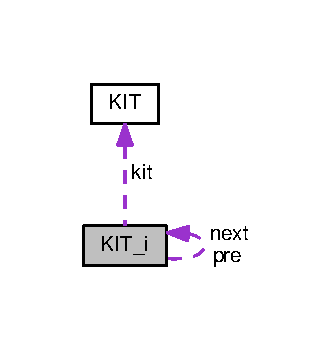
\includegraphics[width=160pt]{structKIT__i__coll__graph}
\end{center}
\end{figure}
\subsection*{Public Attributes}
\begin{DoxyCompactItemize}
\item 
\hypertarget{structKIT__i_a6edcec5a34f35c40b93a2b04e5037e65}{}\hyperlink{structKIT}{K\+I\+T} $\ast$ \hyperlink{structKIT__i_a6edcec5a34f35c40b93a2b04e5037e65}{kit}\label{structKIT__i_a6edcec5a34f35c40b93a2b04e5037e65}

\begin{DoxyCompactList}\small\item\em kit medico \end{DoxyCompactList}\item 
\hypertarget{structKIT__i_aea986829d6c2d2da88cb78b93e5b0ae3}{}\hyperlink{structKIT__i}{K\+I\+T\+\_\+i} $\ast$ \hyperlink{structKIT__i_aea986829d6c2d2da88cb78b93e5b0ae3}{pre}\label{structKIT__i_aea986829d6c2d2da88cb78b93e5b0ae3}

\begin{DoxyCompactList}\small\item\em puntatore al nodo precedente \end{DoxyCompactList}\item 
\hypertarget{structKIT__i_a81d57e322a6b294a56152c8e12afca76}{}\hyperlink{structKIT__i}{K\+I\+T\+\_\+i} $\ast$ \hyperlink{structKIT__i_a81d57e322a6b294a56152c8e12afca76}{next}\label{structKIT__i_a81d57e322a6b294a56152c8e12afca76}

\begin{DoxyCompactList}\small\item\em puntatore al nodo succesivo \end{DoxyCompactList}\end{DoxyCompactItemize}


\subsection{Detailed Description}
Questa struct definisce una lista bidirezionale di kit medici. 

The documentation for this struct was generated from the following file\+:\begin{DoxyCompactItemize}
\item 
\hyperlink{Animazioni_8hpp}{Animazioni.\+hpp}\end{DoxyCompactItemize}

\hypertarget{classLivello}{}\section{Livello Class Reference}
\label{classLivello}\index{Livello@{Livello}}


Definisce le specifiche che deve avere un livello di gioco.  




{\ttfamily \#include $<$Livello.\+hpp$>$}



Collaboration diagram for Livello\+:\nopagebreak
\begin{figure}[H]
\begin{center}
\leavevmode
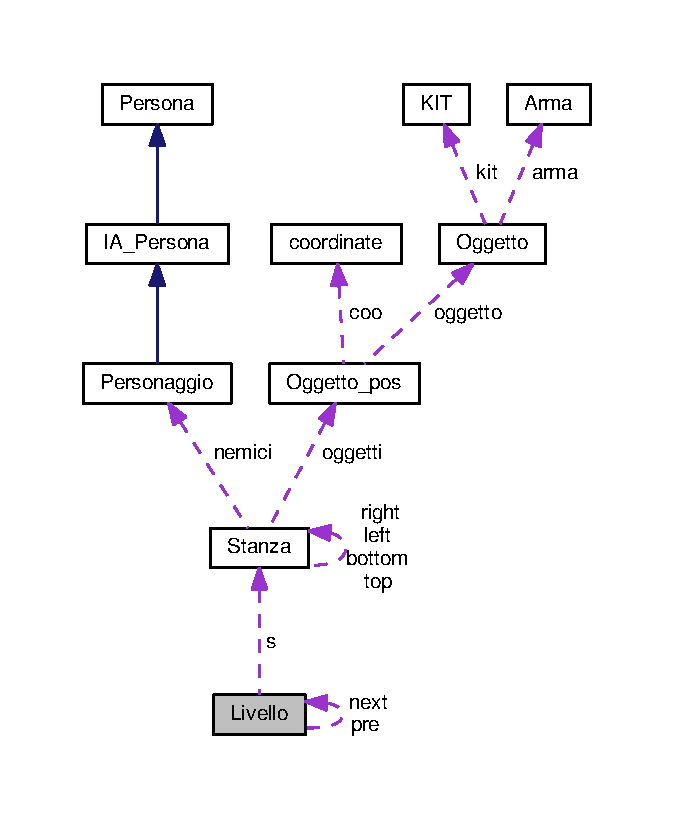
\includegraphics[width=323pt]{classLivello__coll__graph}
\end{center}
\end{figure}
\subsection*{Public Member Functions}
\begin{DoxyCompactItemize}
\item 
\hyperlink{classLivello_ac1d34208a12139365a7eb749a5668f8f}{Livello} (\hyperlink{classGiocatore}{Giocatore} $\ast$gamer, \hyperlink{classLivello}{Livello} $\ast$\hyperlink{classLivello_a05397a3b59545c76f627de49f23d70a8}{pre}, int direction\+\_\+pre\+\_\+stanza, int livello, int num\+\_\+time\+\_\+machine\+\_\+part)
\begin{DoxyCompactList}\small\item\em Costruttore che crea le stanze del livello e genera i pezzi della macchina del tempo. \end{DoxyCompactList}\item 
\hypertarget{classLivello_ac68f1cff83b129ca15659d114d01019e}{}int \hyperlink{classLivello_ac68f1cff83b129ca15659d114d01019e}{get\+N\+Livello} ()\label{classLivello_ac68f1cff83b129ca15659d114d01019e}

\begin{DoxyCompactList}\small\item\em ritorna l\textquotesingle{}indice del livello \end{DoxyCompactList}\item 
void \hyperlink{classLivello_a4b3938ca43f2b73c7d326077f737147a}{set\+Livello} (int livello)
\begin{DoxyCompactList}\small\item\em modifica l\textquotesingle{}indice del livello \end{DoxyCompactList}\item 
\hypertarget{classLivello_a6c9fa17a5a53d8d7f5ee588fb262e204}{}int \hyperlink{classLivello_a6c9fa17a5a53d8d7f5ee588fb262e204}{get\+Num\+Stanze} ()\label{classLivello_a6c9fa17a5a53d8d7f5ee588fb262e204}

\begin{DoxyCompactList}\small\item\em ritorna il numero delle stanze generati per il livello \end{DoxyCompactList}\end{DoxyCompactItemize}
\subsection*{Public Attributes}
\begin{DoxyCompactItemize}
\item 
\hypertarget{classLivello_a601562dc27ce8063d5335afe287a1301}{}\hyperlink{classStanza}{Stanza} $\ast$ \hyperlink{classLivello_a601562dc27ce8063d5335afe287a1301}{s}\label{classLivello_a601562dc27ce8063d5335afe287a1301}

\begin{DoxyCompactList}\small\item\em prima stanza del livello \end{DoxyCompactList}\item 
\hypertarget{classLivello_a787f31d6da22aeaea69f3a2a4603c918}{}\hyperlink{classLivello}{Livello} $\ast$ \hyperlink{classLivello_a787f31d6da22aeaea69f3a2a4603c918}{next}\label{classLivello_a787f31d6da22aeaea69f3a2a4603c918}

\begin{DoxyCompactList}\small\item\em puntatore al livello successivo \end{DoxyCompactList}\item 
\hypertarget{classLivello_a05397a3b59545c76f627de49f23d70a8}{}\hyperlink{classLivello}{Livello} $\ast$ \hyperlink{classLivello_a05397a3b59545c76f627de49f23d70a8}{pre}\label{classLivello_a05397a3b59545c76f627de49f23d70a8}

\begin{DoxyCompactList}\small\item\em puntatore al livello precedente \end{DoxyCompactList}\item 
\hypertarget{classLivello_a9175836818c82d7f13dd47c68f125b0d}{}int \hyperlink{classLivello_a9175836818c82d7f13dd47c68f125b0d}{num\+\_\+stanze}\label{classLivello_a9175836818c82d7f13dd47c68f125b0d}

\begin{DoxyCompactList}\small\item\em numero di stanze generate nel livello ($<$=n\+\_\+stanze) \end{DoxyCompactList}\end{DoxyCompactItemize}


\subsection{Detailed Description}
Definisce le specifiche che deve avere un livello di gioco. 

\subsection{Constructor \& Destructor Documentation}
\hypertarget{classLivello_ac1d34208a12139365a7eb749a5668f8f}{}\index{Livello@{Livello}!Livello@{Livello}}
\index{Livello@{Livello}!Livello@{Livello}}
\subsubsection[{Livello}]{\setlength{\rightskip}{0pt plus 5cm}Livello\+::\+Livello (
\begin{DoxyParamCaption}
\item[{{\bf Giocatore} $\ast$}]{gamer, }
\item[{{\bf Livello} $\ast$}]{pre, }
\item[{int}]{direction\+\_\+pre\+\_\+stanza, }
\item[{int}]{livello, }
\item[{int}]{num\+\_\+time\+\_\+machine\+\_\+part}
\end{DoxyParamCaption}
)}\label{classLivello_ac1d34208a12139365a7eb749a5668f8f}


Costruttore che crea le stanze del livello e genera i pezzi della macchina del tempo. 


\begin{DoxyParams}{Parameters}
{\em gamer} & \hyperlink{classGiocatore}{Giocatore} utente \\
\hline
{\em pre} & \hyperlink{classLivello}{Livello} precedente (=N\+U\+L\+L se è il primo livello, !=N\+U\+L\+L altrimenti) \\
\hline
{\em direction\+\_\+pre\+\_\+stanza} & direzione delle scale dell\textquotesingle{}ultima stanza del livello precedente (4=su,2=giu,1=sx,3,dx) \\
\hline
{\em livello} & indice del livello \\
\hline
{\em num\+\_\+time\+\_\+machine\+\_\+part} & numero di pezzi della macchina del tempo da generare nel livello \\
\hline
\end{DoxyParams}


\subsection{Member Function Documentation}
\hypertarget{classLivello_a4b3938ca43f2b73c7d326077f737147a}{}\index{Livello@{Livello}!set\+Livello@{set\+Livello}}
\index{set\+Livello@{set\+Livello}!Livello@{Livello}}
\subsubsection[{set\+Livello}]{\setlength{\rightskip}{0pt plus 5cm}Livello\+::set\+Livello (
\begin{DoxyParamCaption}
\item[{int}]{livello}
\end{DoxyParamCaption}
)}\label{classLivello_a4b3938ca43f2b73c7d326077f737147a}


modifica l\textquotesingle{}indice del livello 


\begin{DoxyParams}{Parameters}
{\em livello} & nuovo livello \\
\hline
\end{DoxyParams}


The documentation for this class was generated from the following files\+:\begin{DoxyCompactItemize}
\item 
\hyperlink{Livello_8hpp}{Livello.\+hpp}\item 
Livello.\+cpp\end{DoxyCompactItemize}

\hypertarget{structOggetto}{}\section{Oggetto Struct Reference}
\label{structOggetto}\index{Oggetto@{Oggetto}}


Collaboration diagram for Oggetto\+:\nopagebreak
\begin{figure}[H]
\begin{center}
\leavevmode
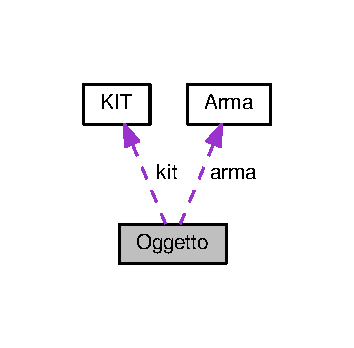
\includegraphics[width=170pt]{structOggetto__coll__graph}
\end{center}
\end{figure}
\subsection*{Public Attributes}
\begin{DoxyCompactItemize}
\item 
\hypertarget{structOggetto_ae58234e8df0dad2e0ab520d5b26224de}{}\hyperlink{structKIT}{K\+I\+T} $\ast$ \hyperlink{structOggetto_ae58234e8df0dad2e0ab520d5b26224de}{kit}\label{structOggetto_ae58234e8df0dad2e0ab520d5b26224de}

\begin{DoxyCompactList}\small\item\em puntatore al kit medico \end{DoxyCompactList}\item 
\hypertarget{structOggetto_af0c4461aacfaa7c0b41ae693cfae193f}{}\hyperlink{classArma}{Arma} $\ast$ \hyperlink{structOggetto_af0c4461aacfaa7c0b41ae693cfae193f}{arma}\label{structOggetto_af0c4461aacfaa7c0b41ae693cfae193f}

\begin{DoxyCompactList}\small\item\em puntatore all\textquotesingle{}arma \end{DoxyCompactList}\end{DoxyCompactItemize}


The documentation for this struct was generated from the following file\+:\begin{DoxyCompactItemize}
\item 
\hyperlink{Persona_8hpp}{Persona.\+hpp}\end{DoxyCompactItemize}

\hypertarget{structOggetto__pos}{}\section{Oggetto\+\_\+pos Struct Reference}
\label{structOggetto__pos}\index{Oggetto\+\_\+pos@{Oggetto\+\_\+pos}}


Questa struct permette l\textquotesingle{}associazione Oggetto-\/coordinate.  




{\ttfamily \#include $<$I\+A\+\_\+\+Persona.\+hpp$>$}



Collaboration diagram for Oggetto\+\_\+pos\+:\nopagebreak
\begin{figure}[H]
\begin{center}
\leavevmode
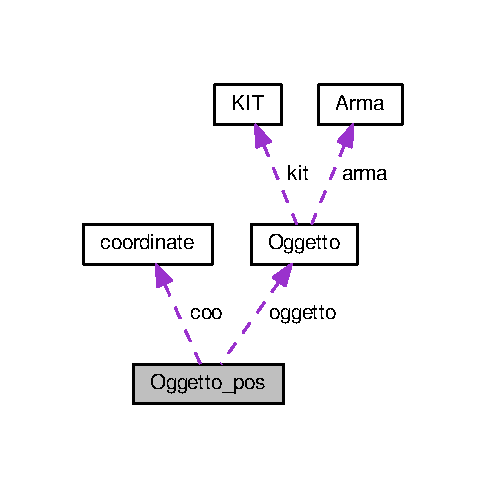
\includegraphics[width=233pt]{structOggetto__pos__coll__graph}
\end{center}
\end{figure}
\subsection*{Public Attributes}
\begin{DoxyCompactItemize}
\item 
\hypertarget{structOggetto__pos_acb0695ca7d62692637a184901d426464}{}\hyperlink{structOggetto}{Oggetto} \hyperlink{structOggetto__pos_acb0695ca7d62692637a184901d426464}{oggetto}\label{structOggetto__pos_acb0695ca7d62692637a184901d426464}

\begin{DoxyCompactList}\small\item\em oggetto raccoglibile \end{DoxyCompactList}\item 
\hypertarget{structOggetto__pos_aee7a056d2f9b14861f48c299d01eaf5f}{}\hyperlink{structcoordinate}{coordinate} \hyperlink{structOggetto__pos_aee7a056d2f9b14861f48c299d01eaf5f}{coo}\label{structOggetto__pos_aee7a056d2f9b14861f48c299d01eaf5f}

\begin{DoxyCompactList}\small\item\em coordinate \end{DoxyCompactList}\end{DoxyCompactItemize}


\subsection{Detailed Description}
Questa struct permette l\textquotesingle{}associazione Oggetto-\/coordinate. 

The documentation for this struct was generated from the following file\+:\begin{DoxyCompactItemize}
\item 
\hyperlink{IA__Persona_8hpp}{I\+A\+\_\+\+Persona.\+hpp}\end{DoxyCompactItemize}

\hypertarget{classPersona}{}\section{Persona Class Reference}
\label{classPersona}\index{Persona@{Persona}}


definisce le caratterische di una persona (che è la classe padre radice di tutte le sue derivate)  




{\ttfamily \#include $<$Persona.\+hpp$>$}



Inheritance diagram for Persona\+:\nopagebreak
\begin{figure}[H]
\begin{center}
\leavevmode
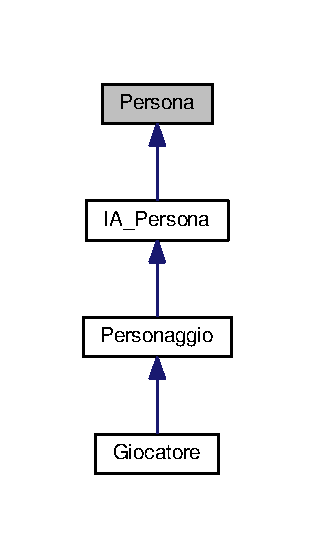
\includegraphics[width=151pt]{classPersona__inherit__graph}
\end{center}
\end{figure}
\subsection*{Public Member Functions}
\begin{DoxyCompactItemize}
\item 
\hyperlink{classPersona_a5e4c7859de8f9284666715dbc5614ccd}{Persona} (char \hyperlink{classPersona_a15d4ded972e8bdd3f02e89c6ccb71b73}{nome}\mbox{[}50\mbox{]}, char \hyperlink{classPersona_ae7069f0467a3b2f1d269c1a143b730eb}{tipo}\mbox{[}50\mbox{]}, int \hyperlink{classPersona_a1e784d3a56cddd6ba8e81387df1efc7b}{vita}, char \hyperlink{classPersona_a1fff44e46be477b79413387307b0aaff}{carattere})
\begin{DoxyCompactList}\small\item\em Costruttore. \end{DoxyCompactList}\item 
void \hyperlink{classPersona_a4bea4b34933c85e2eee8443cdba6a940}{get\+Nome} (char \hyperlink{classPersona_a15d4ded972e8bdd3f02e89c6ccb71b73}{nome}\mbox{[}$\,$\mbox{]})
\begin{DoxyCompactList}\small\item\em ritorna il nome della persona \end{DoxyCompactList}\item 
void \hyperlink{classPersona_a8edc79607b544d69427da678bffbef51}{get\+Tipo} (char \hyperlink{classPersona_ae7069f0467a3b2f1d269c1a143b730eb}{tipo}\mbox{[}$\,$\mbox{]})
\begin{DoxyCompactList}\small\item\em ritorna il tipo della persona \end{DoxyCompactList}\item 
\hypertarget{classPersona_a008f0bc840f0e3e1dd306832f798637b}{}char \hyperlink{classPersona_a008f0bc840f0e3e1dd306832f798637b}{get\+Carattere} ()\label{classPersona_a008f0bc840f0e3e1dd306832f798637b}

\begin{DoxyCompactList}\small\item\em ritorna il carattere della persona \end{DoxyCompactList}\item 
void \hyperlink{classPersona_a9fcee7f1342f27a4c34d8e8275f4ba24}{set\+Carattere} (char \hyperlink{classPersona_a1fff44e46be477b79413387307b0aaff}{carattere})
\begin{DoxyCompactList}\small\item\em Modifica il carattere della persona. \end{DoxyCompactList}\item 
\hypertarget{classPersona_aa28e4ec15979f7a01f71e1c1888e5116}{}bool \hyperlink{classPersona_aa28e4ec15979f7a01f71e1c1888e5116}{get\+Scudo} ()\label{classPersona_aa28e4ec15979f7a01f71e1c1888e5116}

\begin{DoxyCompactList}\small\item\em ritorna lo stato dello scudo \end{DoxyCompactList}\item 
void \hyperlink{classPersona_a20449ddc606a872a8905c94fe0ed716a}{set\+Scudo} (bool \hyperlink{classPersona_a1af99e040deeb7015e7e99bb2a5128f4}{scudo})
\begin{DoxyCompactList}\small\item\em Modifica lo stato dello scudo. \end{DoxyCompactList}\item 
void \hyperlink{classPersona_aeca07343f896b49854a6b3eb7acadf99}{add\+Vita} (int \hyperlink{classPersona_a1e784d3a56cddd6ba8e81387df1efc7b}{vita})
\begin{DoxyCompactList}\small\item\em Aggiunge unità di vita al persona. \end{DoxyCompactList}\item 
void \hyperlink{classPersona_af759e5da9d0972da4a74ce6a56e271aa}{sub\+Vita} (int \hyperlink{classPersona_a1e784d3a56cddd6ba8e81387df1efc7b}{vita})
\begin{DoxyCompactList}\small\item\em Toglie unità di vita al persona. \end{DoxyCompactList}\item 
\hypertarget{classPersona_a7f8f0aa7052c06e40ddbbdd4f62f3c4d}{}int \hyperlink{classPersona_a7f8f0aa7052c06e40ddbbdd4f62f3c4d}{get\+Vita} ()\label{classPersona_a7f8f0aa7052c06e40ddbbdd4f62f3c4d}

\begin{DoxyCompactList}\small\item\em Ritorna le unità di vita della persona. \end{DoxyCompactList}\item 
\hypertarget{classPersona_a537b7f6ab867ce01ab850c378bf30cf4}{}\hyperlink{classArma}{Arma} $\ast$ \hyperlink{classPersona_a537b7f6ab867ce01ab850c378bf30cf4}{get\+Arma} ()\label{classPersona_a537b7f6ab867ce01ab850c378bf30cf4}

\begin{DoxyCompactList}\small\item\em ritona il puntatore all\textquotesingle{}arma corrente della persona \end{DoxyCompactList}\item 
void \hyperlink{classPersona_a60a40a075ceb82c3a5586c589478abe4}{set\+Arma} (\hyperlink{classArma}{Arma} $\ast$arma\+\_\+corrente)
\begin{DoxyCompactList}\small\item\em Modifica l\textquotesingle{}arma corrente del personaggio. \end{DoxyCompactList}\item 
bool \hyperlink{classPersona_a9d2d465914d3fc2e4594cebc4fc3cfb8}{add\+Oggetto} (\hyperlink{structOggetto}{Oggetto} o)
\begin{DoxyCompactList}\small\item\em Aggiunge un\textquotesingle{}oggetto allo zaino. \end{DoxyCompactList}\item 
bool \hyperlink{classPersona_a295caef7835d4a9f631fc5bb21c57ad3}{compare\+Oggetto} (\hyperlink{structOggetto}{Oggetto} o, int i)
\begin{DoxyCompactList}\small\item\em Confronta l\textquotesingle{}oggetto o con quello presente alla posizione i-\/esima dello zaino. \end{DoxyCompactList}\item 
void \hyperlink{classPersona_a8419f8c494f1b626dcde55f1f0bb1f2e}{remove\+Oggetto} (\hyperlink{structOggetto}{Oggetto} o)
\begin{DoxyCompactList}\small\item\em Rivuove (se è possibile) l\textquotesingle{}oggetto o dallo zaino. \end{DoxyCompactList}\item 
int \hyperlink{classPersona_a8ebd8537b8a1877799829c3d7a3242d3}{get\+Index\+Oggetto} (\hyperlink{structOggetto}{Oggetto} o)
\begin{DoxyCompactList}\small\item\em ritorna l\textquotesingle{}indice del vettore a cui corrisponde l\textquotesingle{}oggetto o ($<$0 altrimenti) \end{DoxyCompactList}\item 
void \hyperlink{classPersona_adce1ee94dc798acffb6a2bbd72c70226}{get\+Zaino} (\hyperlink{structOggetto}{p\+\_\+oggetto} new\+Zaino\mbox{[}50\mbox{]})
\begin{DoxyCompactList}\small\item\em ritorna l\textquotesingle{}intero zaino della persona \end{DoxyCompactList}\item 
void \hyperlink{classPersona_a595fabb934aad33a42b33f4d2d2baf91}{set\+Coordinate} (\hyperlink{structcoordinate}{coordinate} coo)
\begin{DoxyCompactList}\small\item\em modifca le coordinate della persona riferite alla stanza \end{DoxyCompactList}\item 
\hypertarget{classPersona_a37f9b4d937362f9d12dc90c56004315c}{}\hyperlink{structcoordinate}{coordinate} \hyperlink{classPersona_a37f9b4d937362f9d12dc90c56004315c}{get\+Coordinate} ()\label{classPersona_a37f9b4d937362f9d12dc90c56004315c}

\begin{DoxyCompactList}\small\item\em Ritorna le coordinate della persona riferite alla stanza. \end{DoxyCompactList}\end{DoxyCompactItemize}
\subsection*{Protected Attributes}
\begin{DoxyCompactItemize}
\item 
\hypertarget{classPersona_a15d4ded972e8bdd3f02e89c6ccb71b73}{}char \hyperlink{classPersona_a15d4ded972e8bdd3f02e89c6ccb71b73}{nome} \mbox{[}50\mbox{]}\label{classPersona_a15d4ded972e8bdd3f02e89c6ccb71b73}

\begin{DoxyCompactList}\small\item\em nome della persona \end{DoxyCompactList}\item 
\hypertarget{classPersona_ae7069f0467a3b2f1d269c1a143b730eb}{}char \hyperlink{classPersona_ae7069f0467a3b2f1d269c1a143b730eb}{tipo} \mbox{[}50\mbox{]}\label{classPersona_ae7069f0467a3b2f1d269c1a143b730eb}

\begin{DoxyCompactList}\small\item\em tipo della persona (Eroe,Aiutante,Nemico) \end{DoxyCompactList}\item 
\hypertarget{classPersona_a1e784d3a56cddd6ba8e81387df1efc7b}{}int \hyperlink{classPersona_a1e784d3a56cddd6ba8e81387df1efc7b}{vita}\label{classPersona_a1e784d3a56cddd6ba8e81387df1efc7b}

\begin{DoxyCompactList}\small\item\em unita di vita della persona \end{DoxyCompactList}\item 
\hypertarget{classPersona_a1fff44e46be477b79413387307b0aaff}{}char \hyperlink{classPersona_a1fff44e46be477b79413387307b0aaff}{carattere}\label{classPersona_a1fff44e46be477b79413387307b0aaff}

\begin{DoxyCompactList}\small\item\em carattere della personache viene stampato a video \end{DoxyCompactList}\item 
\hypertarget{classPersona_a1af99e040deeb7015e7e99bb2a5128f4}{}bool \hyperlink{classPersona_a1af99e040deeb7015e7e99bb2a5128f4}{scudo}\label{classPersona_a1af99e040deeb7015e7e99bb2a5128f4}

\begin{DoxyCompactList}\small\item\em flag che indica se lo scudo della persona è atttivo o meno \end{DoxyCompactList}\end{DoxyCompactItemize}


\subsection{Detailed Description}
definisce le caratterische di una persona (che è la classe padre radice di tutte le sue derivate) 

\subsection{Constructor \& Destructor Documentation}
\hypertarget{classPersona_a5e4c7859de8f9284666715dbc5614ccd}{}\index{Persona@{Persona}!Persona@{Persona}}
\index{Persona@{Persona}!Persona@{Persona}}
\subsubsection[{Persona}]{\setlength{\rightskip}{0pt plus 5cm}Persona\+::\+Persona (
\begin{DoxyParamCaption}
\item[{char}]{nome\mbox{[}50\mbox{]}, }
\item[{char}]{tipo\mbox{[}50\mbox{]}, }
\item[{int}]{vita, }
\item[{char}]{carattere}
\end{DoxyParamCaption}
)}\label{classPersona_a5e4c7859de8f9284666715dbc5614ccd}


Costruttore. 


\begin{DoxyParams}{Parameters}
{\em nome} & nome della persona \\
\hline
{\em tipo} & tipo della persona \\
\hline
{\em vita} & unità di vita della persona \\
\hline
{\em carattere} & carattere stampato a video della persona \\
\hline
\end{DoxyParams}


\subsection{Member Function Documentation}
\hypertarget{classPersona_a9d2d465914d3fc2e4594cebc4fc3cfb8}{}\index{Persona@{Persona}!add\+Oggetto@{add\+Oggetto}}
\index{add\+Oggetto@{add\+Oggetto}!Persona@{Persona}}
\subsubsection[{add\+Oggetto}]{\setlength{\rightskip}{0pt plus 5cm}Persona\+::add\+Oggetto (
\begin{DoxyParamCaption}
\item[{{\bf Oggetto}}]{o}
\end{DoxyParamCaption}
)}\label{classPersona_a9d2d465914d3fc2e4594cebc4fc3cfb8}


Aggiunge un\textquotesingle{}oggetto allo zaino. 


\begin{DoxyParams}{Parameters}
{\em o} & nuovo oggetto da aggiungere. Ritorna true se ha aggiunto o, false altrimenti \\
\hline
\end{DoxyParams}
\hypertarget{classPersona_aeca07343f896b49854a6b3eb7acadf99}{}\index{Persona@{Persona}!add\+Vita@{add\+Vita}}
\index{add\+Vita@{add\+Vita}!Persona@{Persona}}
\subsubsection[{add\+Vita}]{\setlength{\rightskip}{0pt plus 5cm}Persona\+::add\+Vita (
\begin{DoxyParamCaption}
\item[{int}]{vita}
\end{DoxyParamCaption}
)}\label{classPersona_aeca07343f896b49854a6b3eb7acadf99}


Aggiunge unità di vita al persona. 


\begin{DoxyParams}{Parameters}
{\em vita} & quantità da aggiungere \\
\hline
\end{DoxyParams}
\hypertarget{classPersona_a295caef7835d4a9f631fc5bb21c57ad3}{}\index{Persona@{Persona}!compare\+Oggetto@{compare\+Oggetto}}
\index{compare\+Oggetto@{compare\+Oggetto}!Persona@{Persona}}
\subsubsection[{compare\+Oggetto}]{\setlength{\rightskip}{0pt plus 5cm}Persona\+::compare\+Oggetto (
\begin{DoxyParamCaption}
\item[{{\bf Oggetto}}]{o, }
\item[{int}]{i}
\end{DoxyParamCaption}
)}\label{classPersona_a295caef7835d4a9f631fc5bb21c57ad3}


Confronta l\textquotesingle{}oggetto o con quello presente alla posizione i-\/esima dello zaino. 


\begin{DoxyParams}{Parameters}
{\em o} & oggetto da confrontare \\
\hline
{\em i} & indice del confronto \\
\hline
\end{DoxyParams}
\hypertarget{classPersona_a8ebd8537b8a1877799829c3d7a3242d3}{}\index{Persona@{Persona}!get\+Index\+Oggetto@{get\+Index\+Oggetto}}
\index{get\+Index\+Oggetto@{get\+Index\+Oggetto}!Persona@{Persona}}
\subsubsection[{get\+Index\+Oggetto}]{\setlength{\rightskip}{0pt plus 5cm}Persona\+::get\+Index\+Oggetto (
\begin{DoxyParamCaption}
\item[{{\bf Oggetto}}]{o}
\end{DoxyParamCaption}
)}\label{classPersona_a8ebd8537b8a1877799829c3d7a3242d3}


ritorna l\textquotesingle{}indice del vettore a cui corrisponde l\textquotesingle{}oggetto o ($<$0 altrimenti) 


\begin{DoxyParams}{Parameters}
{\em o} & oggetto per cui si vuole conoscere l\textquotesingle{}indice \\
\hline
\end{DoxyParams}
\hypertarget{classPersona_a4bea4b34933c85e2eee8443cdba6a940}{}\index{Persona@{Persona}!get\+Nome@{get\+Nome}}
\index{get\+Nome@{get\+Nome}!Persona@{Persona}}
\subsubsection[{get\+Nome}]{\setlength{\rightskip}{0pt plus 5cm}Persona\+::get\+Nome (
\begin{DoxyParamCaption}
\item[{char}]{nome\mbox{[}$\,$\mbox{]}}
\end{DoxyParamCaption}
)}\label{classPersona_a4bea4b34933c85e2eee8443cdba6a940}


ritorna il nome della persona 


\begin{DoxyParams}{Parameters}
{\em nome} & vettore che conterrà il nome \\
\hline
\end{DoxyParams}
\hypertarget{classPersona_a8edc79607b544d69427da678bffbef51}{}\index{Persona@{Persona}!get\+Tipo@{get\+Tipo}}
\index{get\+Tipo@{get\+Tipo}!Persona@{Persona}}
\subsubsection[{get\+Tipo}]{\setlength{\rightskip}{0pt plus 5cm}Persona\+::get\+Tipo (
\begin{DoxyParamCaption}
\item[{char}]{tipo\mbox{[}$\,$\mbox{]}}
\end{DoxyParamCaption}
)}\label{classPersona_a8edc79607b544d69427da678bffbef51}


ritorna il tipo della persona 


\begin{DoxyParams}{Parameters}
{\em tipo} & vettore che conterrà il tipo \\
\hline
\end{DoxyParams}
\hypertarget{classPersona_adce1ee94dc798acffb6a2bbd72c70226}{}\index{Persona@{Persona}!get\+Zaino@{get\+Zaino}}
\index{get\+Zaino@{get\+Zaino}!Persona@{Persona}}
\subsubsection[{get\+Zaino}]{\setlength{\rightskip}{0pt plus 5cm}Persona\+::get\+Zaino (
\begin{DoxyParamCaption}
\item[{{\bf p\+\_\+oggetto}}]{new\+Zaino\mbox{[}50\mbox{]}}
\end{DoxyParamCaption}
)}\label{classPersona_adce1ee94dc798acffb6a2bbd72c70226}


ritorna l\textquotesingle{}intero zaino della persona 


\begin{DoxyParams}{Parameters}
{\em new\+Zaino} & vettore dello zaino ritornato per indirizzo \\
\hline
\end{DoxyParams}
\hypertarget{classPersona_a8419f8c494f1b626dcde55f1f0bb1f2e}{}\index{Persona@{Persona}!remove\+Oggetto@{remove\+Oggetto}}
\index{remove\+Oggetto@{remove\+Oggetto}!Persona@{Persona}}
\subsubsection[{remove\+Oggetto}]{\setlength{\rightskip}{0pt plus 5cm}Persona\+::remove\+Oggetto (
\begin{DoxyParamCaption}
\item[{{\bf Oggetto}}]{o}
\end{DoxyParamCaption}
)}\label{classPersona_a8419f8c494f1b626dcde55f1f0bb1f2e}


Rivuove (se è possibile) l\textquotesingle{}oggetto o dallo zaino. 


\begin{DoxyParams}{Parameters}
{\em o} & oggetto da rimuovere \\
\hline
\end{DoxyParams}
\hypertarget{classPersona_a60a40a075ceb82c3a5586c589478abe4}{}\index{Persona@{Persona}!set\+Arma@{set\+Arma}}
\index{set\+Arma@{set\+Arma}!Persona@{Persona}}
\subsubsection[{set\+Arma}]{\setlength{\rightskip}{0pt plus 5cm}Persona\+::set\+Arma (
\begin{DoxyParamCaption}
\item[{{\bf Arma} $\ast$}]{arma\+\_\+corrente}
\end{DoxyParamCaption}
)}\label{classPersona_a60a40a075ceb82c3a5586c589478abe4}


Modifica l\textquotesingle{}arma corrente del personaggio. 


\begin{DoxyParams}{Parameters}
{\em arma\+\_\+corrente} & puntatore all\textquotesingle{}nuova arma corrente \\
\hline
\end{DoxyParams}
\hypertarget{classPersona_a9fcee7f1342f27a4c34d8e8275f4ba24}{}\index{Persona@{Persona}!set\+Carattere@{set\+Carattere}}
\index{set\+Carattere@{set\+Carattere}!Persona@{Persona}}
\subsubsection[{set\+Carattere}]{\setlength{\rightskip}{0pt plus 5cm}Persona\+::set\+Carattere (
\begin{DoxyParamCaption}
\item[{char}]{carattere}
\end{DoxyParamCaption}
)}\label{classPersona_a9fcee7f1342f27a4c34d8e8275f4ba24}


Modifica il carattere della persona. 


\begin{DoxyParams}{Parameters}
{\em carattere} & nuovo carattere dell apersona \\
\hline
\end{DoxyParams}
\hypertarget{classPersona_a595fabb934aad33a42b33f4d2d2baf91}{}\index{Persona@{Persona}!set\+Coordinate@{set\+Coordinate}}
\index{set\+Coordinate@{set\+Coordinate}!Persona@{Persona}}
\subsubsection[{set\+Coordinate}]{\setlength{\rightskip}{0pt plus 5cm}Persona\+::set\+Coordinate (
\begin{DoxyParamCaption}
\item[{{\bf coordinate}}]{coo}
\end{DoxyParamCaption}
)}\label{classPersona_a595fabb934aad33a42b33f4d2d2baf91}


modifca le coordinate della persona riferite alla stanza 


\begin{DoxyParams}{Parameters}
{\em coo} & nuove coordinate della persona \\
\hline
\end{DoxyParams}
\hypertarget{classPersona_a20449ddc606a872a8905c94fe0ed716a}{}\index{Persona@{Persona}!set\+Scudo@{set\+Scudo}}
\index{set\+Scudo@{set\+Scudo}!Persona@{Persona}}
\subsubsection[{set\+Scudo}]{\setlength{\rightskip}{0pt plus 5cm}Persona\+::set\+Scudo (
\begin{DoxyParamCaption}
\item[{bool}]{scudo}
\end{DoxyParamCaption}
)}\label{classPersona_a20449ddc606a872a8905c94fe0ed716a}


Modifica lo stato dello scudo. 


\begin{DoxyParams}{Parameters}
{\em scudo} & nuovo stato dello scudo \\
\hline
\end{DoxyParams}
\hypertarget{classPersona_af759e5da9d0972da4a74ce6a56e271aa}{}\index{Persona@{Persona}!sub\+Vita@{sub\+Vita}}
\index{sub\+Vita@{sub\+Vita}!Persona@{Persona}}
\subsubsection[{sub\+Vita}]{\setlength{\rightskip}{0pt plus 5cm}Persona\+::sub\+Vita (
\begin{DoxyParamCaption}
\item[{int}]{vita}
\end{DoxyParamCaption}
)}\label{classPersona_af759e5da9d0972da4a74ce6a56e271aa}


Toglie unità di vita al persona. 


\begin{DoxyParams}{Parameters}
{\em vita} & quantità da togliere \\
\hline
\end{DoxyParams}


The documentation for this class was generated from the following files\+:\begin{DoxyCompactItemize}
\item 
\hyperlink{Persona_8hpp}{Persona.\+hpp}\item 
Persona.\+cpp\end{DoxyCompactItemize}

\hypertarget{classPersonaggio}{}\section{Personaggio Class Reference}
\label{classPersonaggio}\index{Personaggio@{Personaggio}}


Filgia di \hyperlink{classIA__Persona}{I\+A\+\_\+\+Persona}, definisce un metodo per la gestione automatica di aiutanti e nemici.  




{\ttfamily \#include $<$Personaggio.\+hpp$>$}



Inheritance diagram for Personaggio\+:\nopagebreak
\begin{figure}[H]
\begin{center}
\leavevmode
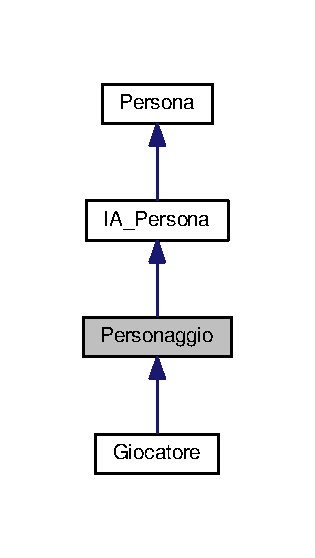
\includegraphics[width=151pt]{classPersonaggio__inherit__graph}
\end{center}
\end{figure}


Collaboration diagram for Personaggio\+:\nopagebreak
\begin{figure}[H]
\begin{center}
\leavevmode
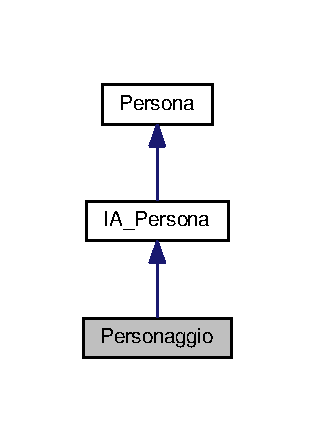
\includegraphics[width=151pt]{classPersonaggio__coll__graph}
\end{center}
\end{figure}
\subsection*{Public Member Functions}
\begin{DoxyCompactItemize}
\item 
\hyperlink{classPersonaggio_ac7577ef8db7274dcb71d91e4572784d2}{Personaggio} (char Nome\mbox{[}50\mbox{]}, char Tipo\mbox{[}50\mbox{]}, char \hyperlink{classPersona_a1fff44e46be477b79413387307b0aaff}{carattere}, int \hyperlink{classPersona_a1e784d3a56cddd6ba8e81387df1efc7b}{vita})
\begin{DoxyCompactList}\small\item\em Costruttore. \end{DoxyCompactList}\item 
void \hyperlink{classPersonaggio_adc6035b95bffaec15a0c879bbc773af6}{Auto\+Action} (\hyperlink{structController}{Controller} $\ast$\hyperlink{structcontroller}{controller}, char stanza\mbox{[}25\mbox{]}\mbox{[}91\mbox{]}, \hyperlink{structcoordinate}{coordinate} coo\+\_\+stanza, \hyperlink{classPersona}{Persona} $\ast$personaggi\mbox{[}$\,$\mbox{]}, int num\+\_\+personaggi, \hyperlink{structOggetto__pos}{Oggetto\+\_\+pos} $\ast$$\ast$oggetti, int num\+\_\+oggetti, int $\ast$total\+\_\+time\+\_\+machine\+\_\+part\+\_\+catched, int local\+\_\+time\+\_\+machine\+\_\+part, \hyperlink{structTime__Machine}{Time\+\_\+\+Machine} $\ast$$\ast$time\+\_\+machine\+\_\+coo)
\begin{DoxyCompactList}\small\item\em permette la gestione automatica del personaggio in questione \end{DoxyCompactList}\end{DoxyCompactItemize}
\subsection*{Additional Inherited Members}


\subsection{Detailed Description}
Filgia di \hyperlink{classIA__Persona}{I\+A\+\_\+\+Persona}, definisce un metodo per la gestione automatica di aiutanti e nemici. 

\subsection{Constructor \& Destructor Documentation}
\hypertarget{classPersonaggio_ac7577ef8db7274dcb71d91e4572784d2}{}\index{Personaggio@{Personaggio}!Personaggio@{Personaggio}}
\index{Personaggio@{Personaggio}!Personaggio@{Personaggio}}
\subsubsection[{Personaggio}]{\setlength{\rightskip}{0pt plus 5cm}Personaggio\+::\+Personaggio (
\begin{DoxyParamCaption}
\item[{char}]{Nome\mbox{[}50\mbox{]}, }
\item[{char}]{Tipo\mbox{[}50\mbox{]}, }
\item[{char}]{carattere, }
\item[{int}]{vita}
\end{DoxyParamCaption}
)}\label{classPersonaggio_ac7577ef8db7274dcb71d91e4572784d2}


Costruttore. 


\begin{DoxyParams}{Parameters}
{\em Nome} & nome della persona \\
\hline
{\em Tipo} & tipo della persona \\
\hline
{\em carattere} & carattere stampato a video della persona \\
\hline
{\em vita} & unità di vita della persona \\
\hline
\end{DoxyParams}


\subsection{Member Function Documentation}
\hypertarget{classPersonaggio_adc6035b95bffaec15a0c879bbc773af6}{}\index{Personaggio@{Personaggio}!Auto\+Action@{Auto\+Action}}
\index{Auto\+Action@{Auto\+Action}!Personaggio@{Personaggio}}
\subsubsection[{Auto\+Action}]{\setlength{\rightskip}{0pt plus 5cm}Personaggio\+::\+Auto\+Action (
\begin{DoxyParamCaption}
\item[{{\bf Controller} $\ast$}]{controller, }
\item[{char}]{stanza\mbox{[}25\mbox{]}\mbox{[}91\mbox{]}, }
\item[{{\bf coordinate}}]{coo\+\_\+stanza, }
\item[{{\bf Persona} $\ast$}]{personaggi\mbox{[}$\,$\mbox{]}, }
\item[{int}]{num\+\_\+personaggi, }
\item[{{\bf Oggetto\+\_\+pos} $\ast$$\ast$}]{oggetti, }
\item[{int}]{num\+\_\+oggetti, }
\item[{int $\ast$}]{total\+\_\+time\+\_\+machine\+\_\+part\+\_\+catched, }
\item[{int}]{local\+\_\+time\+\_\+machine\+\_\+part, }
\item[{{\bf Time\+\_\+\+Machine} $\ast$$\ast$}]{time\+\_\+machine\+\_\+coo}
\end{DoxyParamCaption}
)}\label{classPersonaggio_adc6035b95bffaec15a0c879bbc773af6}


permette la gestione automatica del personaggio in questione 


\begin{DoxyParams}{Parameters}
{\em controller} & struttura dati che rappresenta l\textquotesingle{}insieme dei comandi utente \\
\hline
{\em stanza} & matrice della stanza in cui è presente il giocatore \\
\hline
{\em coo\+\_\+stanza} & coordinate della stanza in questione sullo schermo \\
\hline
{\em personaggi} & vettore di tutte le persone (giocatore, aiutanti e nemici) nella stanza in questione \\
\hline
{\em num\+\_\+personaggi} & lunghezza del vettore personaggi \\
\hline
{\em oggetti} & vettore di tutti gli oggetti raccoglibili nella stanza in questione \\
\hline
{\em num\+\_\+oggetti} & lunghezza del vettore oggetti \\
\hline
{\em total\+\_\+time\+\_\+machine\+\_\+part\+\_\+catched} & numero di pezzi della macchina del tempo attualmente raccolti \\
\hline
{\em local\+\_\+time\+\_\+machine\+\_\+part} & numero di pezzi della macchina del tempo presenti nella stanza corrente \\
\hline
{\em time\+\_\+machine\+\_\+coo} & vettore di \hyperlink{structTime__Machine}{Time\+\_\+\+Machine} \\
\hline
\end{DoxyParams}


The documentation for this class was generated from the following files\+:\begin{DoxyCompactItemize}
\item 
\hyperlink{Personaggio_8hpp}{Personaggio.\+hpp}\item 
Personaggio.\+cpp\end{DoxyCompactItemize}

\hypertarget{structrestore__ch}{}\section{restore\+\_\+ch Struct Reference}
\label{structrestore__ch}\index{restore\+\_\+ch@{restore\+\_\+ch}}


Questa struct definisce i caratteri da ripristinare.  




{\ttfamily \#include $<$Structure.\+hpp$>$}



Collaboration diagram for restore\+\_\+ch\+:\nopagebreak
\begin{figure}[H]
\begin{center}
\leavevmode
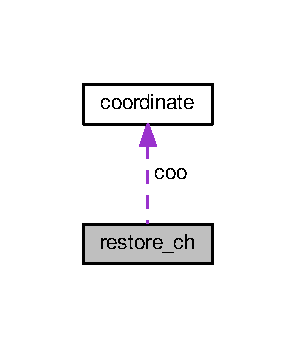
\includegraphics[width=142pt]{structrestore__ch__coll__graph}
\end{center}
\end{figure}
\subsection*{Public Attributes}
\begin{DoxyCompactItemize}
\item 
\hypertarget{structrestore__ch_a25af9707740fb5a85efc89cd95f66698}{}char \hyperlink{structrestore__ch_a25af9707740fb5a85efc89cd95f66698}{ch}\label{structrestore__ch_a25af9707740fb5a85efc89cd95f66698}

\begin{DoxyCompactList}\small\item\em carattere da ripristinare \end{DoxyCompactList}\item 
\hypertarget{structrestore__ch_a7e132144db0a22ede1a5c2d1c5b133ec}{}\hyperlink{structcoordinate}{coordinate} \hyperlink{structrestore__ch_a7e132144db0a22ede1a5c2d1c5b133ec}{coo}\label{structrestore__ch_a7e132144db0a22ede1a5c2d1c5b133ec}

\begin{DoxyCompactList}\small\item\em coordinate del carattere da ripristinare \end{DoxyCompactList}\end{DoxyCompactItemize}


\subsection{Detailed Description}
Questa struct definisce i caratteri da ripristinare. 

The documentation for this struct was generated from the following file\+:\begin{DoxyCompactItemize}
\item 
Structure.\+hpp\end{DoxyCompactItemize}

\hypertarget{classStanza}{}\section{Stanza Class Reference}
\label{classStanza}\index{Stanza@{Stanza}}


defisce le specifiche della stanza di ogni livello di gioco  




{\ttfamily \#include $<$Stanza.\+hpp$>$}



Collaboration diagram for Stanza\+:\nopagebreak
\begin{figure}[H]
\begin{center}
\leavevmode
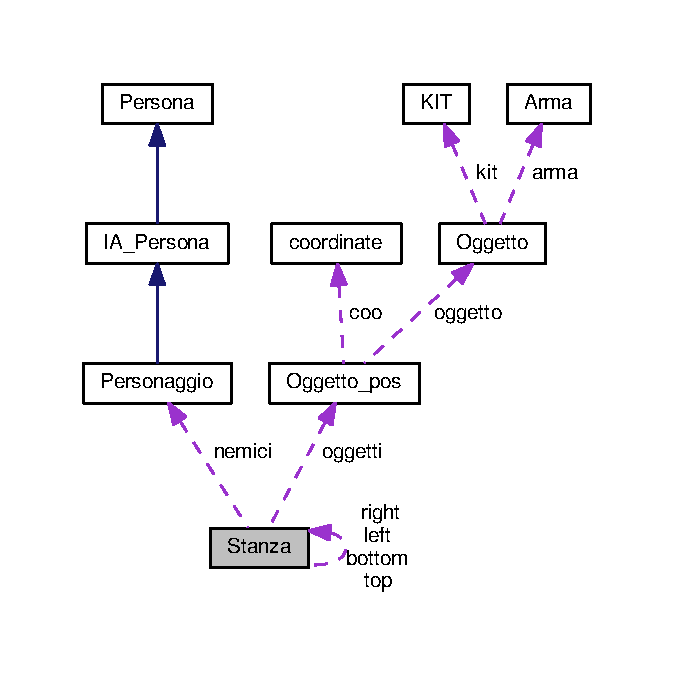
\includegraphics[width=323pt]{classStanza__coll__graph}
\end{center}
\end{figure}
\subsection*{Public Member Functions}
\begin{DoxyCompactItemize}
\item 
void \hyperlink{classStanza_ab2cf3e8b8ff07d0b2e085e811d4bd877}{set\+Index\+Stanza} (int new\+Index)
\begin{DoxyCompactList}\small\item\em modifica l\textquotesingle{}indice della stanza \end{DoxyCompactList}\item 
\hypertarget{classStanza_acb46dd0c2fd4babf46a3e7df63d686e8}{}int \hyperlink{classStanza_acb46dd0c2fd4babf46a3e7df63d686e8}{get\+Index\+Stanza} ()\label{classStanza_acb46dd0c2fd4babf46a3e7df63d686e8}

\begin{DoxyCompactList}\small\item\em Ritorna l\textquotesingle{}indice della stanza. \end{DoxyCompactList}\item 
void \hyperlink{classStanza_a4fa142675917f53dfe48ce5fa1106efc}{set\+Index\+Livello} (int new\+Index)
\begin{DoxyCompactList}\small\item\em modifica l\textquotesingle{}indice del livello \end{DoxyCompactList}\item 
\hypertarget{classStanza_acc5183dd818e4e84d55a67a0c0e15c29}{}int \hyperlink{classStanza_acc5183dd818e4e84d55a67a0c0e15c29}{get\+Index\+Livello} ()\label{classStanza_acc5183dd818e4e84d55a67a0c0e15c29}

\begin{DoxyCompactList}\small\item\em Ritorna l\textquotesingle{}indice dellivello. \end{DoxyCompactList}\item 
void \hyperlink{classStanza_a2f712f06413ec65a642c03022b02d292}{aggiorna\+Aiutanti} (\hyperlink{classGiocatore}{Giocatore} $\ast$giocatore)
\begin{DoxyCompactList}\small\item\em modifica (quando possibile) il numero di aiutanti per il giocatore \mbox{[}chiamato quando si cambia stanza\mbox{]} \end{DoxyCompactList}\item 
\hyperlink{classStanza_aebe5bf4edcd60661ebe64fba556e8336}{Stanza} (\hyperlink{classGiocatore}{Giocatore} $\ast$giocatore, int id\+Livello, int id\+Stanza, int id\+\_\+matrix\+\_\+used\mbox{[}$\,$\mbox{]}, int num\+\_\+id)
\begin{DoxyCompactList}\small\item\em Costruttore. \end{DoxyCompactList}\end{DoxyCompactItemize}
\subsection*{Public Attributes}
\begin{DoxyCompactItemize}
\item 
\hypertarget{classStanza_a8d01d55aec56b48611025064d84e66de}{}char \hyperlink{classStanza_a8d01d55aec56b48611025064d84e66de}{stanza} \mbox{[}\hyperlink{Stanza_8hpp_a6fbfb5f74a35d56ae39aadb31fddc714}{S\+T\+A\+N\+Z\+A\+\_\+\+Y}\mbox{]}\mbox{[}\hyperlink{Stanza_8hpp_a57d21332cfb3a4adb7041c0db1ada16b}{S\+T\+A\+N\+Z\+A\+\_\+\+X}\mbox{]}\label{classStanza_a8d01d55aec56b48611025064d84e66de}

\begin{DoxyCompactList}\small\item\em matrice di caratteri della stanza corrente \end{DoxyCompactList}\item 
\hypertarget{classStanza_a78ad309c46eb00c0cbcae7b58f4721ef}{}\hyperlink{classStanza}{Stanza} $\ast$ \hyperlink{classStanza_a78ad309c46eb00c0cbcae7b58f4721ef}{top}\label{classStanza_a78ad309c46eb00c0cbcae7b58f4721ef}

\begin{DoxyCompactList}\small\item\em puntatore alla stanza sopra quella corrente \end{DoxyCompactList}\item 
\hypertarget{classStanza_a3c20c96e81f625b1c58525a14ca027c3}{}\hyperlink{classStanza}{Stanza} $\ast$ \hyperlink{classStanza_a3c20c96e81f625b1c58525a14ca027c3}{bottom}\label{classStanza_a3c20c96e81f625b1c58525a14ca027c3}

\begin{DoxyCompactList}\small\item\em puntatore alla stanza sotto quella corrente \end{DoxyCompactList}\item 
\hypertarget{classStanza_ab9fa444357627e27fb3227420c1612c8}{}\hyperlink{classStanza}{Stanza} $\ast$ \hyperlink{classStanza_ab9fa444357627e27fb3227420c1612c8}{right}\label{classStanza_ab9fa444357627e27fb3227420c1612c8}

\begin{DoxyCompactList}\small\item\em puntatore alla stanza destra rispetto quella corrente \end{DoxyCompactList}\item 
\hypertarget{classStanza_aa5b25baa5912ff3be6eef823fd795146}{}\hyperlink{classStanza}{Stanza} $\ast$ \hyperlink{classStanza_aa5b25baa5912ff3be6eef823fd795146}{left}\label{classStanza_aa5b25baa5912ff3be6eef823fd795146}

\begin{DoxyCompactList}\small\item\em puntatore alla stanza sinistra rispetto a quella corrente \end{DoxyCompactList}\item 
\hypertarget{classStanza_aea771b438aed5500cc5de7128b983980}{}int \hyperlink{classStanza_aea771b438aed5500cc5de7128b983980}{n\+\_\+oggetti}\label{classStanza_aea771b438aed5500cc5de7128b983980}

\begin{DoxyCompactList}\small\item\em numero di oggetti raccoglibili nella stanza \end{DoxyCompactList}\item 
\hypertarget{classStanza_a6382ef202b181ce7cf10793b8eeea2f3}{}\hyperlink{structOggetto__pos}{Oggetto\+\_\+pos} $\ast$$\ast$ \hyperlink{classStanza_a6382ef202b181ce7cf10793b8eeea2f3}{oggetti}\label{classStanza_a6382ef202b181ce7cf10793b8eeea2f3}

\begin{DoxyCompactList}\small\item\em oggetti raccoglibili nella stanza \end{DoxyCompactList}\item 
\hypertarget{classStanza_a79632b76d7a97af52b5d350825333615}{}int \hyperlink{classStanza_a79632b76d7a97af52b5d350825333615}{num\+\_\+nemici}\label{classStanza_a79632b76d7a97af52b5d350825333615}

\begin{DoxyCompactList}\small\item\em numero di nemici attualmente generati \end{DoxyCompactList}\item 
\hypertarget{classStanza_a95599af893affa58946f48214103915d}{}\hyperlink{classPersonaggio}{Personaggio} $\ast$ \hyperlink{classStanza_a95599af893affa58946f48214103915d}{nemici} \mbox{[}\hyperlink{classStanza_a3ee6dc829044d6b19fa3ef214ffd3ac9}{num\+\_\+max\+\_\+nemici}\mbox{]}\label{classStanza_a95599af893affa58946f48214103915d}

\begin{DoxyCompactList}\small\item\em vettore di nemici presenti (e assenti) della stanza \end{DoxyCompactList}\end{DoxyCompactItemize}
\subsection*{Static Public Attributes}
\begin{DoxyCompactItemize}
\item 
\hypertarget{classStanza_a3ee6dc829044d6b19fa3ef214ffd3ac9}{}static const int \hyperlink{classStanza_a3ee6dc829044d6b19fa3ef214ffd3ac9}{num\+\_\+max\+\_\+nemici} =10\label{classStanza_a3ee6dc829044d6b19fa3ef214ffd3ac9}

\begin{DoxyCompactList}\small\item\em numero massimo di nemici generabili per la stanza \end{DoxyCompactList}\end{DoxyCompactItemize}


\subsection{Detailed Description}
defisce le specifiche della stanza di ogni livello di gioco 

Definizione della struttura \hyperlink{structOggetto__pos}{Oggetto\+\_\+pos}. 

\subsection{Constructor \& Destructor Documentation}
\hypertarget{classStanza_aebe5bf4edcd60661ebe64fba556e8336}{}\index{Stanza@{Stanza}!Stanza@{Stanza}}
\index{Stanza@{Stanza}!Stanza@{Stanza}}
\subsubsection[{Stanza}]{\setlength{\rightskip}{0pt plus 5cm}Stanza\+::\+Stanza (
\begin{DoxyParamCaption}
\item[{{\bf Giocatore} $\ast$}]{giocatore, }
\item[{int}]{id\+Livello, }
\item[{int}]{id\+Stanza, }
\item[{int}]{id\+\_\+matrix\+\_\+used\mbox{[}$\,$\mbox{]}, }
\item[{int}]{num\+\_\+id}
\end{DoxyParamCaption}
)}\label{classStanza_aebe5bf4edcd60661ebe64fba556e8336}


Costruttore. 


\begin{DoxyParams}{Parameters}
{\em giocatore} & Indica il giocatore (umano) presente nella stanza \\
\hline
{\em id\+Livello} & Indice del livello della stanza \\
\hline
{\em id\+Stanza} & Indice della stanza per uno specifico livello \\
\hline
\end{DoxyParams}


\subsection{Member Function Documentation}
\hypertarget{classStanza_a2f712f06413ec65a642c03022b02d292}{}\index{Stanza@{Stanza}!aggiorna\+Aiutanti@{aggiorna\+Aiutanti}}
\index{aggiorna\+Aiutanti@{aggiorna\+Aiutanti}!Stanza@{Stanza}}
\subsubsection[{aggiorna\+Aiutanti}]{\setlength{\rightskip}{0pt plus 5cm}Stanza\+::aggiorna\+Aiutanti (
\begin{DoxyParamCaption}
\item[{{\bf Giocatore} $\ast$}]{giocatore}
\end{DoxyParamCaption}
)}\label{classStanza_a2f712f06413ec65a642c03022b02d292}


modifica (quando possibile) il numero di aiutanti per il giocatore \mbox{[}chiamato quando si cambia stanza\mbox{]} 


\begin{DoxyParams}{Parameters}
{\em giocatore} & Indica il giocatore a cui aggiornare i propri aiutanti \\
\hline
\end{DoxyParams}
\hypertarget{classStanza_a4fa142675917f53dfe48ce5fa1106efc}{}\index{Stanza@{Stanza}!set\+Index\+Livello@{set\+Index\+Livello}}
\index{set\+Index\+Livello@{set\+Index\+Livello}!Stanza@{Stanza}}
\subsubsection[{set\+Index\+Livello}]{\setlength{\rightskip}{0pt plus 5cm}Stanza\+::set\+Index\+Livello (
\begin{DoxyParamCaption}
\item[{int}]{new\+Index}
\end{DoxyParamCaption}
)}\label{classStanza_a4fa142675917f53dfe48ce5fa1106efc}


modifica l\textquotesingle{}indice del livello 


\begin{DoxyParams}{Parameters}
{\em new\+Index} & nuovo indice del livello della stanza \\
\hline
\end{DoxyParams}
\hypertarget{classStanza_ab2cf3e8b8ff07d0b2e085e811d4bd877}{}\index{Stanza@{Stanza}!set\+Index\+Stanza@{set\+Index\+Stanza}}
\index{set\+Index\+Stanza@{set\+Index\+Stanza}!Stanza@{Stanza}}
\subsubsection[{set\+Index\+Stanza}]{\setlength{\rightskip}{0pt plus 5cm}Stanza\+::set\+Index\+Stanza (
\begin{DoxyParamCaption}
\item[{int}]{new\+Index}
\end{DoxyParamCaption}
)}\label{classStanza_ab2cf3e8b8ff07d0b2e085e811d4bd877}


modifica l\textquotesingle{}indice della stanza 


\begin{DoxyParams}{Parameters}
{\em new\+Index} & nuovo indice della stanza \\
\hline
\end{DoxyParams}


The documentation for this class was generated from the following files\+:\begin{DoxyCompactItemize}
\item 
\hyperlink{Stanza_8hpp}{Stanza.\+hpp}\item 
Stanza.\+cpp\end{DoxyCompactItemize}

\hypertarget{structTime__Machine}{}\section{Time\+\_\+\+Machine Struct Reference}
\label{structTime__Machine}\index{Time\+\_\+\+Machine@{Time\+\_\+\+Machine}}


Questa struct definisce un oggetto raccoglibile (kit medico o arma). Può essere definito solo uno dei due puntatori.  




{\ttfamily \#include $<$Persona.\+hpp$>$}



Collaboration diagram for Time\+\_\+\+Machine\+:\nopagebreak
\begin{figure}[H]
\begin{center}
\leavevmode
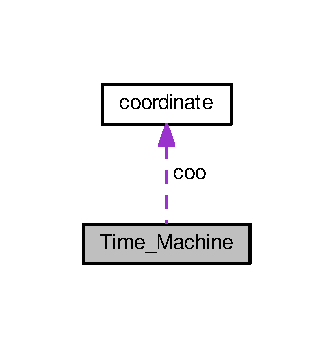
\includegraphics[width=160pt]{structTime__Machine__coll__graph}
\end{center}
\end{figure}
\subsection*{Public Attributes}
\begin{DoxyCompactItemize}
\item 
\hypertarget{structTime__Machine_a3493421879269b494d0c622ab362864d}{}\hyperlink{structcoordinate}{coordinate} {\bfseries coo}\label{structTime__Machine_a3493421879269b494d0c622ab362864d}

\item 
\hypertarget{structTime__Machine_a7758931499204635bc529bf0411f74bc}{}bool {\bfseries trovato}\label{structTime__Machine_a7758931499204635bc529bf0411f74bc}

\end{DoxyCompactItemize}


\subsection{Detailed Description}
Questa struct definisce un oggetto raccoglibile (kit medico o arma). Può essere definito solo uno dei due puntatori. 

The documentation for this struct was generated from the following file\+:\begin{DoxyCompactItemize}
\item 
\hyperlink{IA__Persona_8hpp}{I\+A\+\_\+\+Persona.\+hpp}\end{DoxyCompactItemize}

\hypertarget{structTurno}{}\section{Turno Struct Reference}
\label{structTurno}\index{Turno@{Turno}}


Collaboration diagram for Turno\+:\nopagebreak
\begin{figure}[H]
\begin{center}
\leavevmode
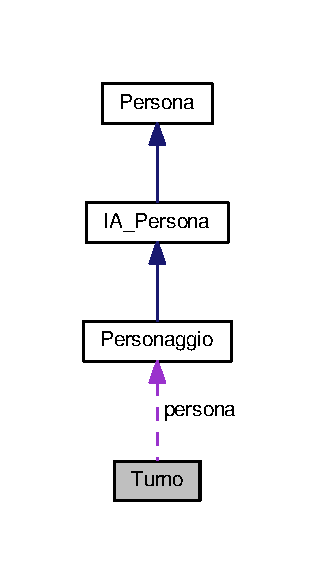
\includegraphics[width=153pt]{structTurno__coll__graph}
\end{center}
\end{figure}
\subsection*{Public Attributes}
\begin{DoxyCompactItemize}
\item 
\hypertarget{structTurno_ab77100d524ed9ee84e72a95f910e5d8d}{}\hyperlink{classPersonaggio}{Personaggio} $\ast$ {\bfseries persona}\label{structTurno_ab77100d524ed9ee84e72a95f910e5d8d}

\item 
\hypertarget{structTurno_ae46461bb7036c1062144ec467f62921c}{}bool {\bfseries turno}\label{structTurno_ae46461bb7036c1062144ec467f62921c}

\end{DoxyCompactItemize}


The documentation for this struct was generated from the following file\+:\begin{DoxyCompactItemize}
\item 
Game.\+hpp\end{DoxyCompactItemize}

\chapter{File Documentation}
\hypertarget{Animazioni_8hpp}{}\section{Animazioni.\+hpp File Reference}
\label{Animazioni_8hpp}\index{Animazioni.\+hpp@{Animazioni.\+hpp}}
{\ttfamily \#include \char`\"{}Livello.\+hpp\char`\"{}}\\*
{\ttfamily \#include \char`\"{}Structure.\+hpp\char`\"{}}\\*
Include dependency graph for Animazioni.\+hpp\+:\nopagebreak
\begin{figure}[H]
\begin{center}
\leavevmode
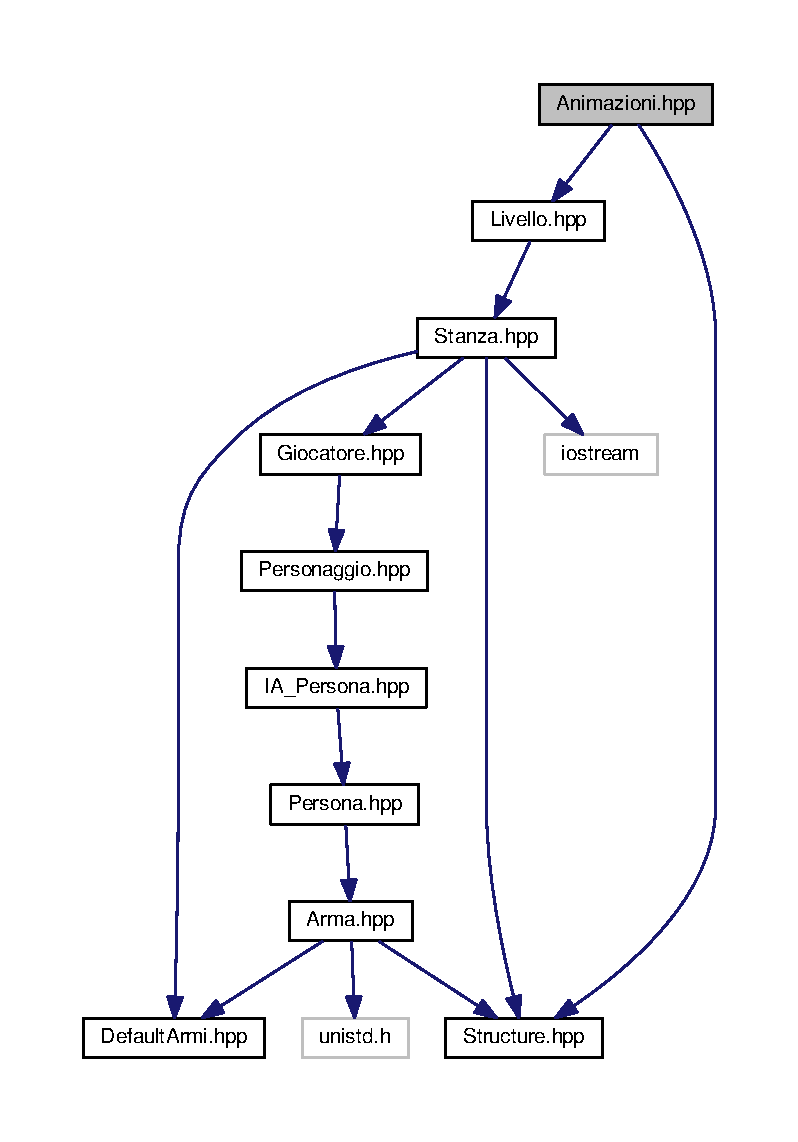
\includegraphics[width=350pt]{Animazioni_8hpp__incl}
\end{center}
\end{figure}
This graph shows which files directly or indirectly include this file\+:\nopagebreak
\begin{figure}[H]
\begin{center}
\leavevmode
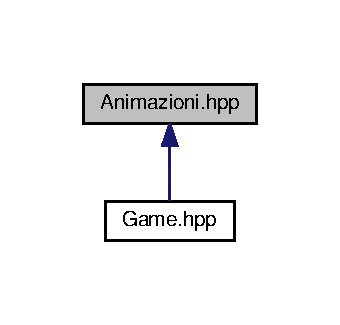
\includegraphics[width=163pt]{Animazioni_8hpp__dep__incl}
\end{center}
\end{figure}
\subsection*{Classes}
\begin{DoxyCompactItemize}
\item 
struct \hyperlink{structArma__i}{Arma\+\_\+i}
\begin{DoxyCompactList}\small\item\em Questa struct definisce una lista bidirezionale di armi con la rispettiva picture. \end{DoxyCompactList}\item 
struct \hyperlink{structKIT__i}{K\+I\+T\+\_\+i}
\begin{DoxyCompactList}\small\item\em Questa struct definisce una lista bidirezionale di kit medici. \end{DoxyCompactList}\item 
class \hyperlink{classAnimazioni}{Animazioni}
\begin{DoxyCompactList}\small\item\em Gestisce le principali animazioni del gioco. \end{DoxyCompactList}\end{DoxyCompactItemize}
\subsection*{Typedefs}
\begin{DoxyCompactItemize}
\item 
\hypertarget{Animazioni_8hpp_ac079d23bc4eadcf6b9df81b92470ec55}{}typedef \hyperlink{structArma__i}{Arma\+\_\+i} $\ast$ {\bfseries Arma\+\_\+icon}\label{Animazioni_8hpp_ac079d23bc4eadcf6b9df81b92470ec55}

\item 
\hypertarget{Animazioni_8hpp_a157c7b69302219f55bdc3c965aec4c5c}{}typedef \hyperlink{structKIT__i}{K\+I\+T\+\_\+i} $\ast$ {\bfseries K\+I\+T\+\_\+icon}\label{Animazioni_8hpp_a157c7b69302219f55bdc3c965aec4c5c}

\end{DoxyCompactItemize}


\subsection{Detailed Description}
\begin{DoxyAuthor}{Author}
Francesco Palmisano 
\end{DoxyAuthor}

\hypertarget{Arma_8hpp}{}\section{Arma.\+hpp File Reference}
\label{Arma_8hpp}\index{Arma.\+hpp@{Arma.\+hpp}}
{\ttfamily \#include $<$unistd.\+h$>$}\\*
{\ttfamily \#include \char`\"{}Structure.\+hpp\char`\"{}}\\*
{\ttfamily \#include \char`\"{}Default\+Armi.\+hpp\char`\"{}}\\*
Include dependency graph for Arma.\+hpp\+:\nopagebreak
\begin{figure}[H]
\begin{center}
\leavevmode
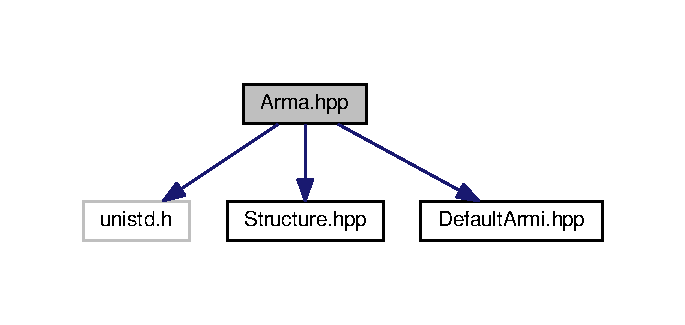
\includegraphics[width=329pt]{Arma_8hpp__incl}
\end{center}
\end{figure}
This graph shows which files directly or indirectly include this file\+:\nopagebreak
\begin{figure}[H]
\begin{center}
\leavevmode
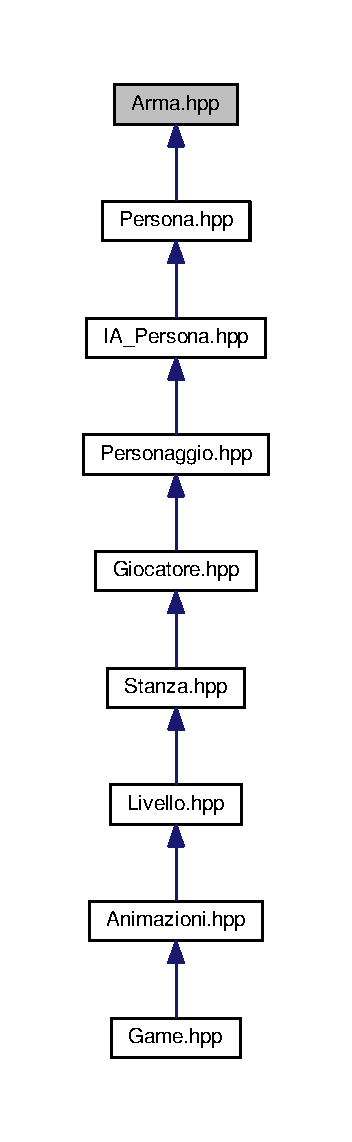
\includegraphics[width=169pt]{Arma_8hpp__dep__incl}
\end{center}
\end{figure}
\subsection*{Classes}
\begin{DoxyCompactItemize}
\item 
class \hyperlink{classArma}{Arma}
\begin{DoxyCompactList}\small\item\em questa classe definisce le specifiche dell\textquotesingle{}arma dei personaggi \end{DoxyCompactList}\end{DoxyCompactItemize}


\subsection{Detailed Description}
\begin{DoxyAuthor}{Author}
Francesco Palmisano 
\end{DoxyAuthor}

\hypertarget{DefaultArmi_8hpp}{}\section{Default\+Armi.\+hpp File Reference}
\label{DefaultArmi_8hpp}\index{Default\+Armi.\+hpp@{Default\+Armi.\+hpp}}
This graph shows which files directly or indirectly include this file\+:\nopagebreak
\begin{figure}[H]
\begin{center}
\leavevmode
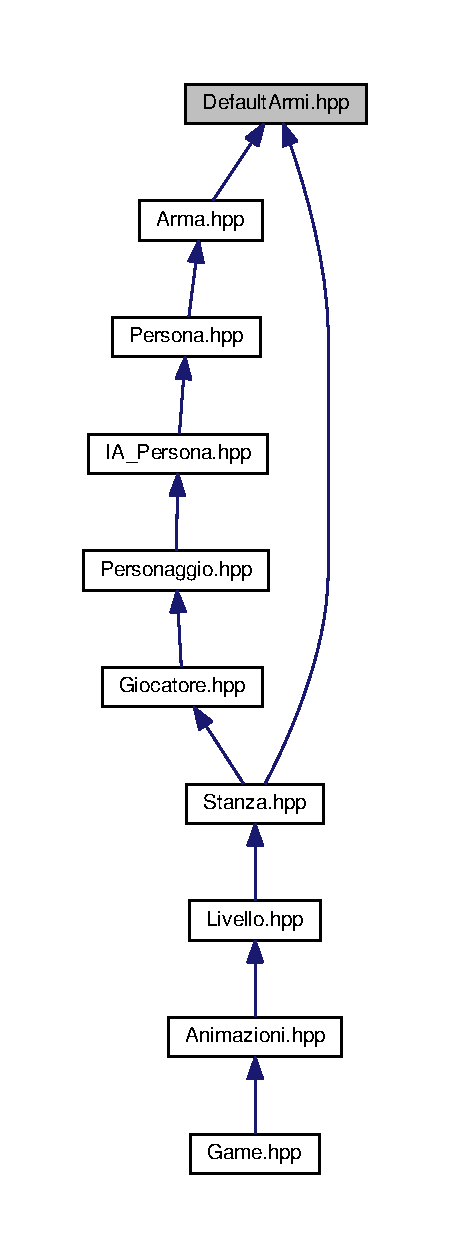
\includegraphics[height=550pt]{DefaultArmi_8hpp__dep__incl}
\end{center}
\end{figure}
\subsection*{Macros}
\begin{DoxyCompactItemize}
\item 
\hypertarget{DefaultArmi_8hpp_ad1408909caf1c8f885c8ab4939ceec0b}{}\#define {\bfseries G\+L\+O\+C\+K45\+\_\+\+M\+U\+N\+I\+Z\+I\+O\+N\+I}~40\label{DefaultArmi_8hpp_ad1408909caf1c8f885c8ab4939ceec0b}

\item 
\hypertarget{DefaultArmi_8hpp_a79262da1dd270014157515a5616ec540}{}\#define {\bfseries G\+L\+O\+C\+K45\+\_\+\+M\+U\+N\+I\+Z\+I\+O\+N\+I\+\_\+\+P\+E\+R\+\_\+\+S\+P\+A\+R\+O}~1\label{DefaultArmi_8hpp_a79262da1dd270014157515a5616ec540}

\item 
\hypertarget{DefaultArmi_8hpp_a733de5b672fce4c000b642f9af1fd442}{}\#define {\bfseries G\+L\+O\+C\+K45\+\_\+\+D\+A\+N\+N\+I}~15\label{DefaultArmi_8hpp_a733de5b672fce4c000b642f9af1fd442}

\item 
\hypertarget{DefaultArmi_8hpp_a731102d4e7ff2a711e767c2d199d8dc7}{}\#define {\bfseries G\+L\+O\+C\+K45\+\_\+\+G\+I\+T\+T\+A\+T\+A}~10\label{DefaultArmi_8hpp_a731102d4e7ff2a711e767c2d199d8dc7}

\item 
\hypertarget{DefaultArmi_8hpp_aeefb7ba38c6800c62a733861541c0a27}{}\#define {\bfseries G\+L\+O\+C\+K45\+\_\+\+I\+D}~1\label{DefaultArmi_8hpp_aeefb7ba38c6800c62a733861541c0a27}

\item 
\hypertarget{DefaultArmi_8hpp_a2815e4e80b3c483b77e3b774c77d0cb3}{}\#define {\bfseries M\+A\+G\+N\+U\+M44\+\_\+\+M\+U\+N\+I\+Z\+I\+O\+N\+I}~30\label{DefaultArmi_8hpp_a2815e4e80b3c483b77e3b774c77d0cb3}

\item 
\hypertarget{DefaultArmi_8hpp_a41c441d0112c04a1e8817a9aae99df02}{}\#define {\bfseries M\+A\+G\+N\+U\+M44\+\_\+\+M\+U\+N\+I\+Z\+I\+O\+N\+I\+\_\+\+P\+E\+R\+\_\+\+S\+P\+A\+R\+O}~1\label{DefaultArmi_8hpp_a41c441d0112c04a1e8817a9aae99df02}

\item 
\hypertarget{DefaultArmi_8hpp_aa34e3402b14bdad0f881026e53139c8b}{}\#define {\bfseries M\+A\+G\+N\+U\+M44\+\_\+\+D\+A\+N\+N\+I}~10\label{DefaultArmi_8hpp_aa34e3402b14bdad0f881026e53139c8b}

\item 
\hypertarget{DefaultArmi_8hpp_ac537a38807c54684c652c281e928a9d0}{}\#define {\bfseries M\+A\+G\+N\+U\+M44\+\_\+\+G\+I\+T\+T\+A\+T\+A}~15\label{DefaultArmi_8hpp_ac537a38807c54684c652c281e928a9d0}

\item 
\hypertarget{DefaultArmi_8hpp_a663dc9bb0134e1b0c2ee167e97addce3}{}\#define {\bfseries M\+A\+G\+N\+U\+M44\+\_\+\+I\+D}~2\label{DefaultArmi_8hpp_a663dc9bb0134e1b0c2ee167e97addce3}

\item 
\hypertarget{DefaultArmi_8hpp_aefcae34b915f2fded4822d845749fbfe}{}\#define {\bfseries M\+A\+C\+H\+I\+N\+E\+G\+U\+N\+\_\+\+M\+U\+N\+I\+Z\+I\+O\+N\+I}~100\label{DefaultArmi_8hpp_aefcae34b915f2fded4822d845749fbfe}

\item 
\hypertarget{DefaultArmi_8hpp_ae57451a4a448f737b64309170b26f3c3}{}\#define {\bfseries M\+A\+C\+H\+I\+N\+E\+G\+U\+N\+\_\+\+M\+U\+N\+I\+Z\+I\+O\+N\+I\+\_\+\+P\+E\+R\+\_\+\+S\+P\+A\+R\+O}~20\label{DefaultArmi_8hpp_ae57451a4a448f737b64309170b26f3c3}

\item 
\hypertarget{DefaultArmi_8hpp_a4d3630913ee3bc343368887103b9bb88}{}\#define {\bfseries M\+A\+C\+H\+I\+N\+E\+G\+U\+N\+\_\+\+D\+A\+N\+N\+I}~5\label{DefaultArmi_8hpp_a4d3630913ee3bc343368887103b9bb88}

\item 
\hypertarget{DefaultArmi_8hpp_a407fb303ebe3212770ebad4975a6041e}{}\#define {\bfseries M\+A\+C\+H\+I\+N\+E\+G\+U\+N\+\_\+\+G\+I\+T\+T\+A\+T\+A}~20\label{DefaultArmi_8hpp_a407fb303ebe3212770ebad4975a6041e}

\item 
\hypertarget{DefaultArmi_8hpp_a6cfad9cca3c83cf0196e336d63374b0f}{}\#define {\bfseries M\+A\+C\+H\+I\+N\+E\+G\+U\+N\+\_\+\+I\+D}~3\label{DefaultArmi_8hpp_a6cfad9cca3c83cf0196e336d63374b0f}

\item 
\hypertarget{DefaultArmi_8hpp_ae35f6475b37557191517e144f7670846}{}\#define {\bfseries A\+K\+\_\+47\+\_\+\+M\+U\+N\+I\+Z\+I\+O\+N\+I}~60\label{DefaultArmi_8hpp_ae35f6475b37557191517e144f7670846}

\item 
\hypertarget{DefaultArmi_8hpp_a692bed3f714164e27bf671c55dbcd049}{}\#define {\bfseries A\+K\+\_\+47\+\_\+\+M\+U\+N\+I\+Z\+I\+O\+N\+I\+\_\+\+P\+E\+R\+\_\+\+S\+P\+A\+R\+O}~5\label{DefaultArmi_8hpp_a692bed3f714164e27bf671c55dbcd049}

\item 
\hypertarget{DefaultArmi_8hpp_a244cb8b5e62af4196149558224e648bb}{}\#define {\bfseries A\+K\+\_\+47\+\_\+\+D\+A\+N\+N\+I}~10\label{DefaultArmi_8hpp_a244cb8b5e62af4196149558224e648bb}

\item 
\hypertarget{DefaultArmi_8hpp_a25a379cc76d4ae31a45b6d160c778d34}{}\#define {\bfseries A\+K\+\_\+47\+\_\+\+G\+I\+T\+T\+A\+T\+A}~23\label{DefaultArmi_8hpp_a25a379cc76d4ae31a45b6d160c778d34}

\item 
\hypertarget{DefaultArmi_8hpp_a62b2f00113a38f42871c37da59e2d822}{}\#define {\bfseries A\+K\+\_\+47\+\_\+\+I\+D}~4\label{DefaultArmi_8hpp_a62b2f00113a38f42871c37da59e2d822}

\item 
\hypertarget{DefaultArmi_8hpp_aea7d99230dd024a02b90f2ee8139d49c}{}\#define {\bfseries W\+A\+R\+F\+A\+R\+E\+\_\+\+S\+N\+I\+P\+E\+R\+\_\+\+M\+U\+N\+I\+Z\+I\+O\+N\+I}~30\label{DefaultArmi_8hpp_aea7d99230dd024a02b90f2ee8139d49c}

\item 
\hypertarget{DefaultArmi_8hpp_a8a24c4fc67a816eabbd02e7f49d1e113}{}\#define {\bfseries W\+A\+R\+F\+A\+R\+E\+\_\+\+S\+N\+I\+P\+E\+R\+\_\+\+M\+U\+N\+I\+Z\+I\+O\+N\+I\+\_\+\+P\+E\+R\+\_\+\+S\+P\+A\+R\+O}~1\label{DefaultArmi_8hpp_a8a24c4fc67a816eabbd02e7f49d1e113}

\item 
\hypertarget{DefaultArmi_8hpp_ac054354e073671e4f157131711bdc94c}{}\#define {\bfseries W\+A\+R\+F\+A\+R\+E\+\_\+\+S\+N\+I\+P\+E\+R\+\_\+\+D\+A\+N\+N\+I}~30\label{DefaultArmi_8hpp_ac054354e073671e4f157131711bdc94c}

\item 
\hypertarget{DefaultArmi_8hpp_aa7e9e1a3b81e6a9853b66bb881c59ea5}{}\#define {\bfseries W\+A\+R\+F\+A\+R\+E\+\_\+\+S\+N\+I\+P\+E\+R\+\_\+\+G\+I\+T\+T\+A\+T\+A}~23\label{DefaultArmi_8hpp_aa7e9e1a3b81e6a9853b66bb881c59ea5}

\item 
\hypertarget{DefaultArmi_8hpp_a23da52e037b072a5ce2c4b964c07d266}{}\#define {\bfseries W\+A\+R\+F\+A\+R\+E\+\_\+\+S\+N\+I\+P\+E\+R\+\_\+\+I\+D}~5\label{DefaultArmi_8hpp_a23da52e037b072a5ce2c4b964c07d266}

\end{DoxyCompactItemize}
\subsection*{Variables}
\begin{DoxyCompactItemize}
\item 
\hypertarget{DefaultArmi_8hpp_a548bff11f7b6e027096f058f554b700a}{}char \hyperlink{DefaultArmi_8hpp_a548bff11f7b6e027096f058f554b700a}{P\+R\+O\+I\+E\+T\+T\+I\+L\+E} =\textquotesingle{}-\/\textquotesingle{}\label{DefaultArmi_8hpp_a548bff11f7b6e027096f058f554b700a}

\begin{DoxyCompactList}\small\item\em carattere comune per tuti i proiettili delle armi \end{DoxyCompactList}\item 
\hypertarget{DefaultArmi_8hpp_a5019367648412af16d38e752407156ac}{}char \hyperlink{DefaultArmi_8hpp_a5019367648412af16d38e752407156ac}{G\+L\+O\+C\+K45} \mbox{[}$\,$\mbox{]} =\char`\"{}glock-\/45\char`\"{}\label{DefaultArmi_8hpp_a5019367648412af16d38e752407156ac}

\begin{DoxyCompactList}\small\item\em nome dell\textquotesingle{}arma \end{DoxyCompactList}\item 
\hypertarget{DefaultArmi_8hpp_ab4c11b8d40e596ec5681b1c1147b0ef0}{}char \hyperlink{DefaultArmi_8hpp_ab4c11b8d40e596ec5681b1c1147b0ef0}{M\+A\+G\+N\+U\+M44} \mbox{[}$\,$\mbox{]} =\char`\"{}44-\/magnum\char`\"{}\label{DefaultArmi_8hpp_ab4c11b8d40e596ec5681b1c1147b0ef0}

\begin{DoxyCompactList}\small\item\em nome dell\textquotesingle{}arma \end{DoxyCompactList}\item 
\hypertarget{DefaultArmi_8hpp_a1d10c6407e660622b291370e5573fa24}{}char \hyperlink{DefaultArmi_8hpp_a1d10c6407e660622b291370e5573fa24}{M\+A\+C\+H\+I\+N\+E\+G\+U\+N} \mbox{[}$\,$\mbox{]} =\char`\"{}machine-\/gun\char`\"{}\label{DefaultArmi_8hpp_a1d10c6407e660622b291370e5573fa24}

\begin{DoxyCompactList}\small\item\em nome dell\textquotesingle{}arma \end{DoxyCompactList}\item 
\hypertarget{DefaultArmi_8hpp_a5e9401d62c3fec764842ce459f3ccbc7}{}char \hyperlink{DefaultArmi_8hpp_a5e9401d62c3fec764842ce459f3ccbc7}{A\+K\+\_\+47} \mbox{[}$\,$\mbox{]} =\char`\"{}ak-\/47\char`\"{}\label{DefaultArmi_8hpp_a5e9401d62c3fec764842ce459f3ccbc7}

\begin{DoxyCompactList}\small\item\em nome dell\textquotesingle{}arma \end{DoxyCompactList}\item 
\hypertarget{DefaultArmi_8hpp_a3f0d7c1b428945289f46ce3a457a0f0b}{}char \hyperlink{DefaultArmi_8hpp_a3f0d7c1b428945289f46ce3a457a0f0b}{W\+A\+R\+F\+A\+R\+E\+\_\+\+S\+N\+I\+P\+E\+R} \mbox{[}$\,$\mbox{]} =\char`\"{}warfare sniper\char`\"{}\label{DefaultArmi_8hpp_a3f0d7c1b428945289f46ce3a457a0f0b}

\begin{DoxyCompactList}\small\item\em nome dell\textquotesingle{}arma \end{DoxyCompactList}\end{DoxyCompactItemize}


\subsection{Detailed Description}
\begin{DoxyAuthor}{Author}
Francesco Palmisano 
\end{DoxyAuthor}

\hypertarget{Giocatore_8hpp}{}\section{Giocatore.\+hpp File Reference}
\label{Giocatore_8hpp}\index{Giocatore.\+hpp@{Giocatore.\+hpp}}
{\ttfamily \#include \char`\"{}Personaggio.\+hpp\char`\"{}}\\*
Include dependency graph for Giocatore.\+hpp\+:\nopagebreak
\begin{figure}[H]
\begin{center}
\leavevmode
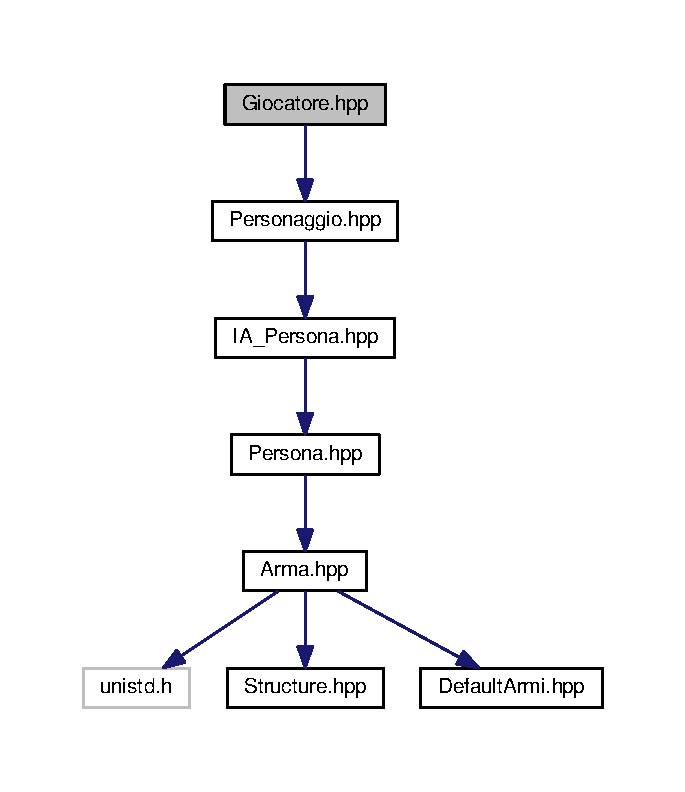
\includegraphics[width=329pt]{Giocatore_8hpp__incl}
\end{center}
\end{figure}
This graph shows which files directly or indirectly include this file\+:\nopagebreak
\begin{figure}[H]
\begin{center}
\leavevmode
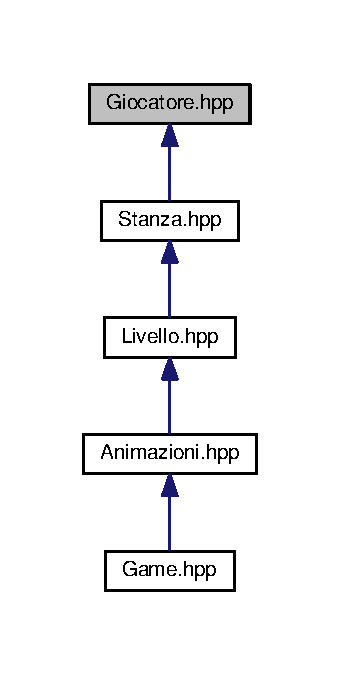
\includegraphics[width=163pt]{Giocatore_8hpp__dep__incl}
\end{center}
\end{figure}
\subsection*{Classes}
\begin{DoxyCompactItemize}
\item 
class \hyperlink{classGiocatore}{Giocatore}
\begin{DoxyCompactList}\small\item\em Figlia di \hyperlink{classPersona}{Persona} definisce le specifiche aggiuntive del giocatore utente. \end{DoxyCompactList}\end{DoxyCompactItemize}


\subsection{Detailed Description}
\begin{DoxyAuthor}{Author}
Luca Tabanelli 
\end{DoxyAuthor}

\hypertarget{IA__Persona_8hpp}{}\section{I\+A\+\_\+\+Persona.\+hpp File Reference}
\label{IA__Persona_8hpp}\index{I\+A\+\_\+\+Persona.\+hpp@{I\+A\+\_\+\+Persona.\+hpp}}
{\ttfamily \#include \char`\"{}Persona.\+hpp\char`\"{}}\\*
Include dependency graph for I\+A\+\_\+\+Persona.\+hpp\+:\nopagebreak
\begin{figure}[H]
\begin{center}
\leavevmode
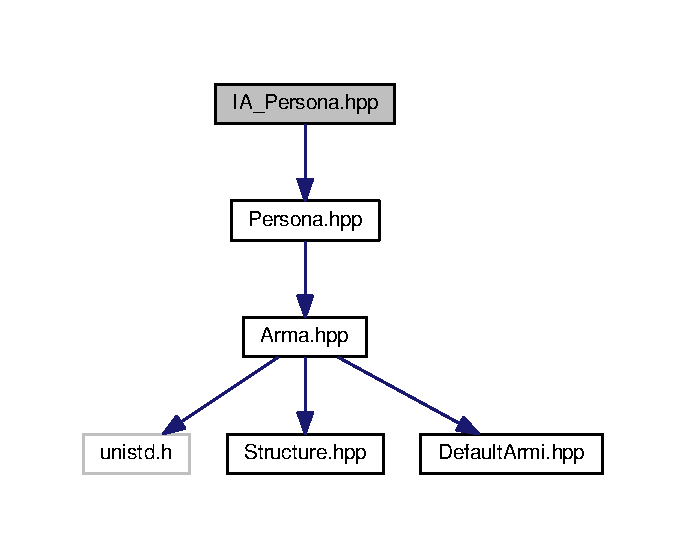
\includegraphics[width=329pt]{IA__Persona_8hpp__incl}
\end{center}
\end{figure}
This graph shows which files directly or indirectly include this file\+:\nopagebreak
\begin{figure}[H]
\begin{center}
\leavevmode
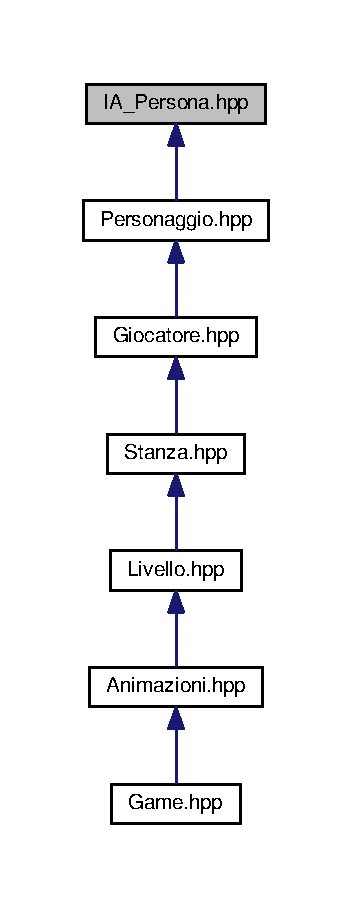
\includegraphics[width=169pt]{IA__Persona_8hpp__dep__incl}
\end{center}
\end{figure}
\subsection*{Classes}
\begin{DoxyCompactItemize}
\item 
struct \hyperlink{structTime__Machine}{Time\+\_\+\+Machine}
\begin{DoxyCompactList}\small\item\em Questa struct definisce un oggetto raccoglibile (kit medico o arma). Può essere definito solo uno dei due puntatori. \end{DoxyCompactList}\item 
struct \hyperlink{structOggetto__pos}{Oggetto\+\_\+pos}
\begin{DoxyCompactList}\small\item\em Questa struct permette l\textquotesingle{}associazione Oggetto-\/coordinate. \end{DoxyCompactList}\item 
class \hyperlink{classIA__Persona}{I\+A\+\_\+\+Persona}
\begin{DoxyCompactList}\small\item\em Gestisce tutte le azioni che vengono considerate come azioni del turno di gioco. \end{DoxyCompactList}\end{DoxyCompactItemize}


\subsection{Detailed Description}
\begin{DoxyAuthor}{Author}
Francesco Palmisano 
\end{DoxyAuthor}

\hypertarget{Livello_8hpp}{}\section{Livello.\+hpp File Reference}
\label{Livello_8hpp}\index{Livello.\+hpp@{Livello.\+hpp}}
{\ttfamily \#include \char`\"{}Stanza.\+hpp\char`\"{}}\\*
Include dependency graph for Livello.\+hpp\+:\nopagebreak
\begin{figure}[H]
\begin{center}
\leavevmode
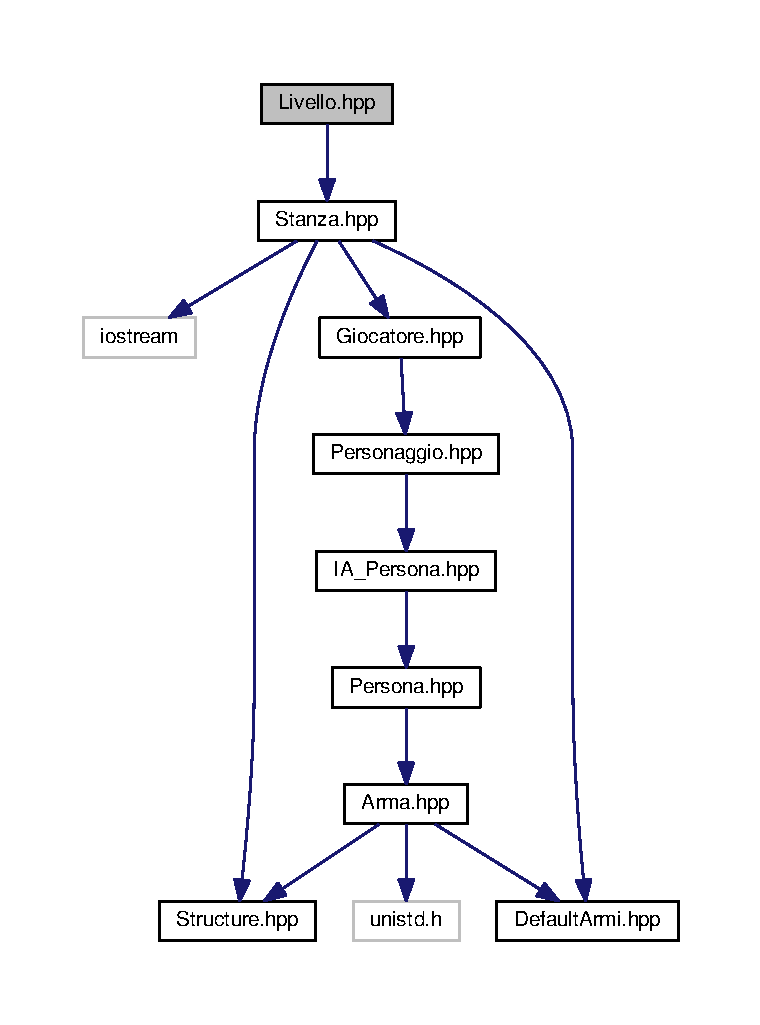
\includegraphics[width=350pt]{Livello_8hpp__incl}
\end{center}
\end{figure}
This graph shows which files directly or indirectly include this file\+:\nopagebreak
\begin{figure}[H]
\begin{center}
\leavevmode
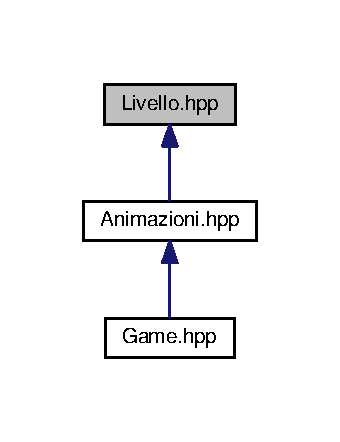
\includegraphics[width=163pt]{Livello_8hpp__dep__incl}
\end{center}
\end{figure}
\subsection*{Classes}
\begin{DoxyCompactItemize}
\item 
class \hyperlink{classLivello}{Livello}
\begin{DoxyCompactList}\small\item\em Definisce le specifiche che deve avere un livello di gioco. \end{DoxyCompactList}\end{DoxyCompactItemize}


\subsection{Detailed Description}
\begin{DoxyAuthor}{Author}
Nicola Serra 
\end{DoxyAuthor}

\hypertarget{Persona_8hpp}{}\section{Persona.\+hpp File Reference}
\label{Persona_8hpp}\index{Persona.\+hpp@{Persona.\+hpp}}
{\ttfamily \#include \char`\"{}Arma.\+hpp\char`\"{}}\\*
Include dependency graph for Persona.\+hpp\+:\nopagebreak
\begin{figure}[H]
\begin{center}
\leavevmode
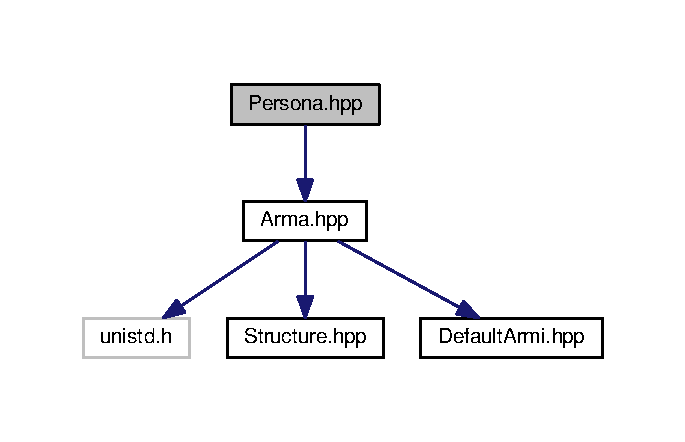
\includegraphics[width=329pt]{Persona_8hpp__incl}
\end{center}
\end{figure}
This graph shows which files directly or indirectly include this file\+:\nopagebreak
\begin{figure}[H]
\begin{center}
\leavevmode
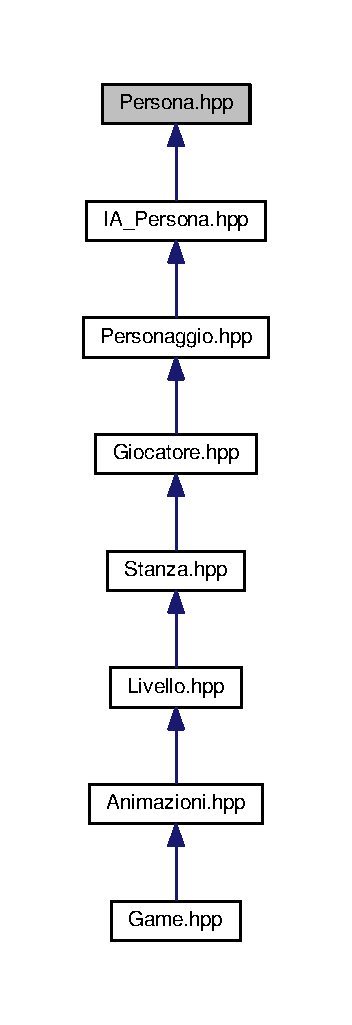
\includegraphics[width=169pt]{Persona_8hpp__dep__incl}
\end{center}
\end{figure}
\subsection*{Classes}
\begin{DoxyCompactItemize}
\item 
struct \hyperlink{structOggetto}{Oggetto}
\item 
class \hyperlink{classPersona}{Persona}
\begin{DoxyCompactList}\small\item\em definisce le caratterische di una persona (che è la classe padre radice di tutte le sue derivate) \end{DoxyCompactList}\end{DoxyCompactItemize}
\subsection*{Typedefs}
\begin{DoxyCompactItemize}
\item 
\hypertarget{Persona_8hpp_a7b80ac2e8b0086288ffc0186e9eb519d}{}typedef \hyperlink{structOggetto}{Oggetto} $\ast$ {\bfseries p\+\_\+oggetto}\label{Persona_8hpp_a7b80ac2e8b0086288ffc0186e9eb519d}

\end{DoxyCompactItemize}


\subsection{Detailed Description}
\begin{DoxyAuthor}{Author}
Luca Tabanelli 
\end{DoxyAuthor}

\hypertarget{Personaggio_8hpp}{}\section{Personaggio.\+hpp File Reference}
\label{Personaggio_8hpp}\index{Personaggio.\+hpp@{Personaggio.\+hpp}}
{\ttfamily \#include \char`\"{}I\+A\+\_\+\+Persona.\+hpp\char`\"{}}\\*
Include dependency graph for Personaggio.\+hpp\+:\nopagebreak
\begin{figure}[H]
\begin{center}
\leavevmode
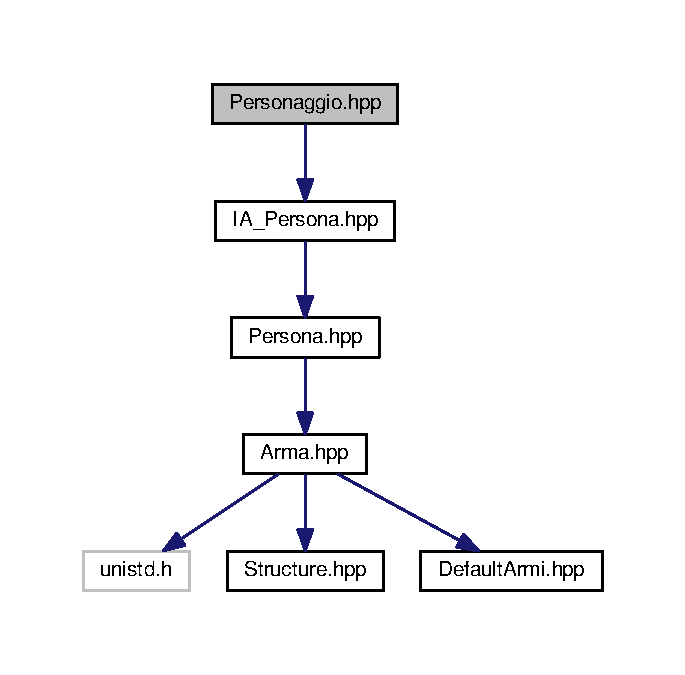
\includegraphics[width=329pt]{Personaggio_8hpp__incl}
\end{center}
\end{figure}
This graph shows which files directly or indirectly include this file\+:\nopagebreak
\begin{figure}[H]
\begin{center}
\leavevmode
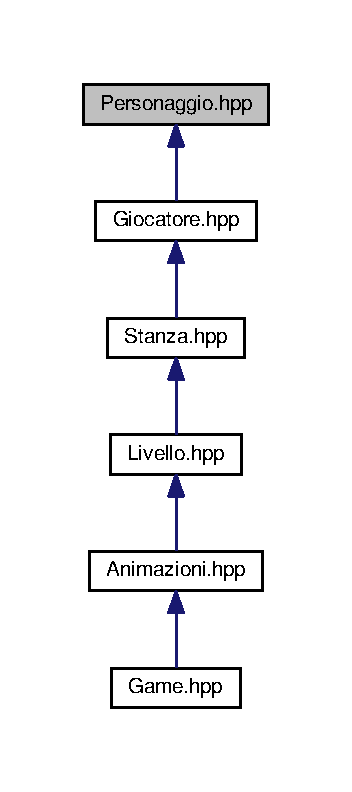
\includegraphics[width=169pt]{Personaggio_8hpp__dep__incl}
\end{center}
\end{figure}
\subsection*{Classes}
\begin{DoxyCompactItemize}
\item 
class \hyperlink{classPersonaggio}{Personaggio}
\begin{DoxyCompactList}\small\item\em Filgia di \hyperlink{classIA__Persona}{I\+A\+\_\+\+Persona}, definisce un metodo per la gestione automatica di aiutanti e nemici. \end{DoxyCompactList}\end{DoxyCompactItemize}


\subsection{Detailed Description}
\begin{DoxyAuthor}{Author}
Luca Tabanelli 
\end{DoxyAuthor}

\hypertarget{Stanza_8hpp}{}\section{Stanza.\+hpp File Reference}
\label{Stanza_8hpp}\index{Stanza.\+hpp@{Stanza.\+hpp}}
{\ttfamily \#include $<$iostream$>$}\\*
{\ttfamily \#include \char`\"{}Giocatore.\+hpp\char`\"{}}\\*
{\ttfamily \#include \char`\"{}Structure.\+hpp\char`\"{}}\\*
{\ttfamily \#include \char`\"{}Default\+Armi.\+hpp\char`\"{}}\\*
Include dependency graph for Stanza.\+hpp\+:\nopagebreak
\begin{figure}[H]
\begin{center}
\leavevmode
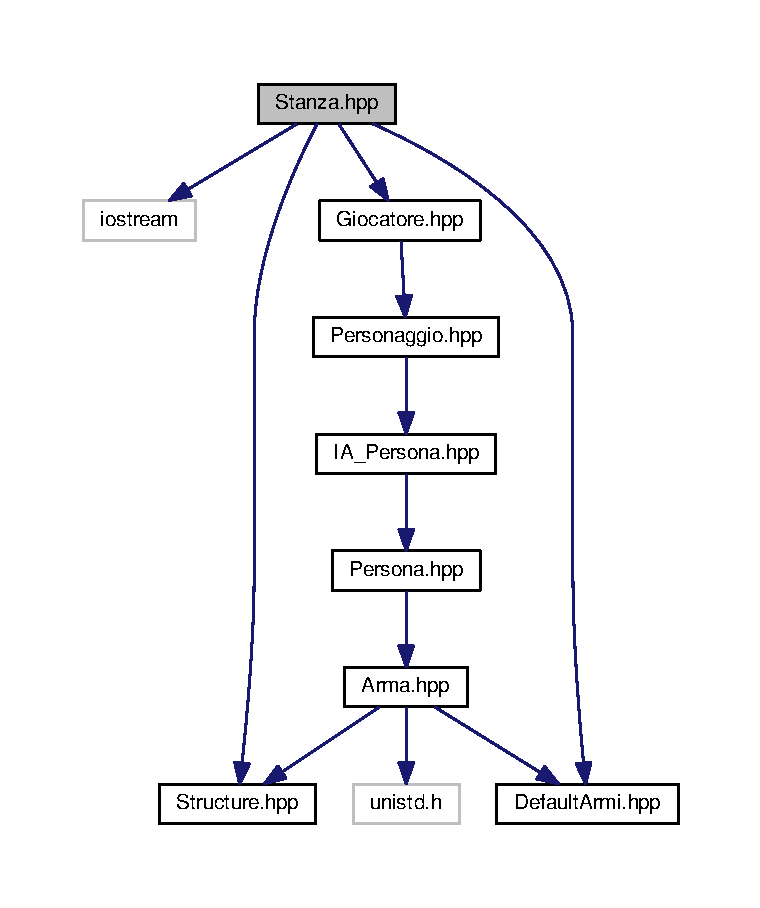
\includegraphics[width=350pt]{Stanza_8hpp__incl}
\end{center}
\end{figure}
This graph shows which files directly or indirectly include this file\+:\nopagebreak
\begin{figure}[H]
\begin{center}
\leavevmode
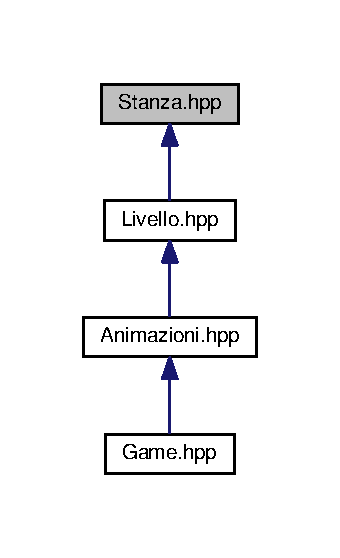
\includegraphics[width=163pt]{Stanza_8hpp__dep__incl}
\end{center}
\end{figure}
\subsection*{Classes}
\begin{DoxyCompactItemize}
\item 
class \hyperlink{classStanza}{Stanza}
\begin{DoxyCompactList}\small\item\em defisce le specifiche della stanza di ogni livello di gioco \end{DoxyCompactList}\end{DoxyCompactItemize}
\subsection*{Macros}
\begin{DoxyCompactItemize}
\item 
\#define \hyperlink{Stanza_8hpp_a57d21332cfb3a4adb7041c0db1ada16b}{S\+T\+A\+N\+Z\+A\+\_\+\+X}~91
\item 
\#define \hyperlink{Stanza_8hpp_a6fbfb5f74a35d56ae39aadb31fddc714}{S\+T\+A\+N\+Z\+A\+\_\+\+Y}~25
\end{DoxyCompactItemize}


\subsection{Detailed Description}
\begin{DoxyAuthor}{Author}
Nicola Serra 
\end{DoxyAuthor}


\subsection{Macro Definition Documentation}
\hypertarget{Stanza_8hpp_a57d21332cfb3a4adb7041c0db1ada16b}{}\index{Stanza.\+hpp@{Stanza.\+hpp}!S\+T\+A\+N\+Z\+A\+\_\+\+X@{S\+T\+A\+N\+Z\+A\+\_\+\+X}}
\index{S\+T\+A\+N\+Z\+A\+\_\+\+X@{S\+T\+A\+N\+Z\+A\+\_\+\+X}!Stanza.\+hpp@{Stanza.\+hpp}}
\subsubsection[{S\+T\+A\+N\+Z\+A\+\_\+\+X}]{\setlength{\rightskip}{0pt plus 5cm}\#define S\+T\+A\+N\+Z\+A\+\_\+\+X~91}\label{Stanza_8hpp_a57d21332cfb3a4adb7041c0db1ada16b}
colonne massimo per stanza \hypertarget{Stanza_8hpp_a6fbfb5f74a35d56ae39aadb31fddc714}{}\index{Stanza.\+hpp@{Stanza.\+hpp}!S\+T\+A\+N\+Z\+A\+\_\+\+Y@{S\+T\+A\+N\+Z\+A\+\_\+\+Y}}
\index{S\+T\+A\+N\+Z\+A\+\_\+\+Y@{S\+T\+A\+N\+Z\+A\+\_\+\+Y}!Stanza.\+hpp@{Stanza.\+hpp}}
\subsubsection[{S\+T\+A\+N\+Z\+A\+\_\+\+Y}]{\setlength{\rightskip}{0pt plus 5cm}\#define S\+T\+A\+N\+Z\+A\+\_\+\+Y~25}\label{Stanza_8hpp_a6fbfb5f74a35d56ae39aadb31fddc714}
righe massime per stanza. 
%--- End generated contents ---

% Index
\backmatter
\newpage
\phantomsection
\clearemptydoublepage
\addcontentsline{toc}{chapter}{Index}
\printindex

\end{document}
